
\documentclass[11pt]{article}
\usepackage[margin=1in]{geometry}

% Core packages
\usepackage{amsmath,amssymb}
\usepackage{tikz-cd}
\usetikzlibrary{arrows.meta,positioning}
\usepackage{multicol}
\usepackage[numbers]{natbib}

% Paragraphs
\setlength{\parindent}{0pt}
\setlength{\parskip}{1\baselineskip}

\title{Optimal Bridge Bidding as a Dynamical Game}
\author{Anders Hansson}
\date{\today}

\begin{document}
\maketitle

\begin{abstract}
This paper develops a rigorous background and research program for computational contract-bridge bidding. It surveys bridge agents, imperfect-information game solving, decentralized-team methods, learning, search, and evaluation. The bidding phase is formalized as a finite-horizon partially observed zero-sum game in which each partnership uses an ex-ante-correlated distribution over complete local bidding plans. The model defines legal auctions, observations, terminal contracts, and reproducible double-dummy raw-score rewards, while distinguishing this self-contained objective from IMP and matchpoint objectives that require comparison mechanisms. The paper explains why benchmark strength and self-play do not establish equilibrium, identifies open theoretical and experimental problems, and specifies the abstractions, response procedures, evaluation protocols, infrastructure, and interpretability tests needed for further research. It does not claim to solve full-scale optimal bridge bidding.
\end{abstract}


\section{Introduction}

Contract bridge is a four-player \emph{imperfect-information game}: some information relevant to the result, most importantly the other players' cards, is hidden from each player. Two partnerships compete over a sequence of deals. The bidding phase is especially interesting from the point of view of game theory and artificial intelligence: each call is both a strategic action and a communication signal to one's partner, while the opponents may interfere with that communication. A \emph{bidding policy} is a rule that assigns a legal call, or probabilities over legal calls, to each hand and auction history that a player can observe. This paper studies the problem of finding an optimal bidding policy in contract bridge. A \emph{state} is a mathematical description of the current situation. The first step is to formulate the bidding phase as a \emph{finite-horizon partially observed Markov game}: a game with finitely many decision times in which a hidden state determines outcomes, each player observes only part of that state, and each player's action may affect later decisions and rewards.

The survey below uses several game-solving terms before their formal mathematical treatment in Appendix~A. A \emph{payoff} is a numerical result that a player or partnership seeks to maximize. A \emph{strategy} is a player's policy in a game. A \emph{best response} is a strategy that maximizes a player or partnership's expected payoff against fixed opposing strategies. An \emph{equilibrium} is a strategy profile in which every participant is using a best response. In a \emph{zero-sum game}, one side's payoff is the negative of the other side's payoff. \emph{Exploitability} measures how much a best response can improve against a candidate strategy, and an \emph{equilibrium certificate} is a valid bound on this improvement. An \emph{extensive-form game} represents sequential decisions by a tree of histories. An \emph{information set} groups histories that a player cannot distinguish, and \emph{perfect recall} means that a player remembers its earlier information and actions.

A \emph{belief} is a probability distribution over hidden states or private information conditional on what has been observed. \emph{Monte Carlo estimation} approximates an expectation by averaging random samples. A \emph{model-based} method uses specified or learned rules for transitions, observations, or other players, whereas a \emph{model-free} method learns values or policies without first constructing those rules explicitly. \emph{Online search} performs additional computation when an action must be selected; the policy available before that computation is called a \emph{blueprint}. \emph{Double-dummy evaluation} evaluates bridge play while treating all four hands as visible.

A \emph{parameterized function} is a function determined by a vector of adjustable numerical parameters. \emph{Supervised learning} fits such a function to supplied input--target pairs, and \emph{imitation learning} uses actions from a person or another program as the targets. A \emph{trajectory} is one complete sequence of states, actions, and rewards. \emph{Reinforcement learning} updates policies or value estimates from generated trajectories and rewards. An \emph{action-value function} assigns an expected future return to an action in a specified situation. \emph{Q-learning} updates such action values toward observed rewards and estimated continuation values. A \emph{policy-gradient method} directly adjusts policy parameters to increase expected return, and \emph{Proximal Policy Optimization} (PPO) is a policy-gradient method that uses a clipped objective to discourage overly large policy-ratio improvements during an update. \emph{Self-play} generates training games using policies produced by the same learning procedure. A saved policy is a \emph{checkpoint}, and a \emph{policy population} is a collection of current or saved policies.

A \emph{decentralized team} contains players that share an objective but choose actions from different private information. A \emph{correlated team strategy} samples a joint plan before private information is observed, whereas independent randomization samples each teammate's plan separately. A \emph{coordinated best response} optimizes all teammates' policies jointly. \emph{Regret} compares accumulated payoff with the payoff from a fixed alternative decision; a \emph{no-regret method} makes average regret approach zero. \emph{Counterfactual regret minimization} (CFR) applies this idea separately at the information sets of an extensive-form game. A \emph{response oracle} constructs an exact or approximate best response, and \emph{Policy-Space Response Oracles} (PSRO) repeatedly adds such responses to policy populations and solves the resulting finite game. Appendix~A gives precise definitions and formulas for these concepts and for the additional named methods used below.

The computational question has several layers that should not be conflated. One is empirical: which methods have actually been tried for bridge bidding? A second is comparative: which methods have succeeded in other zero-sum games with hidden information? A third is theoretical: which algorithms are known to compute or approximate equilibria in partially observed stochastic games and extensive-form games, even when no particular game is the application? Bridge also belongs to a more specialized class than the usual two-player zero-sum model, because each side is a decentralized team whose members have different private information. Throughout the paper, a \emph{model} is a mathematical specification of the relevant players, information, actions, transitions, and objectives; a \emph{program} is a software implementation; a \emph{computational system} is a program together with the policies, models, and search procedures it uses; and a \emph{bidding convention} is an agreed interpretation of calls and their continuations.

Section 2 surveys these four perspectives and ends with a prioritized experimental program. Section 3 then defines the bidding problem precisely. Sections 4 and 5 specify the terminal reward and its consequences for evaluation. Appendix A develops, from first principles, the mathematical definitions behind the game models, equilibrium concepts, learning methods, search procedures, and evaluation criteria used throughout the paper. The purpose of putting the survey before the formal model is to identify which parts of the bridge problem are already addressed by existing methods and which parts require a bridge-specific combination of equilibrium computation, decentralized cooperation, belief inference, function approximation, and search.


\section{Algorithmic Landscape}

\subsection{Computational methods used for bridge}

The bridge literature began with hand-engineered rules, planning, search, and simulation. Much of the early computational work concerned card play rather than bidding, but it established two ideas that remain central. Frank and Basin showed why treating an incomplete-information game as a collection of unrelated perfect-information positions can give strategically inconsistent decisions \cite{frank1998search}. Ginsberg's GIB program combined sampling of possible deals, partition search, and double-dummy evaluation \cite{ginsberg2001gib}. The same basic decomposition later reappears in bidding methods: infer or sample hidden hands, evaluate contracts under a play model, and choose a call using an approximate continuation policy.

Amit and Markovitch gave an early learning-and-search treatment aimed directly at bidding \cite{amit2006learning}. Their method used models of both partner and opponents, model-based Monte Carlo sampling for hidden cards, and co-training in which partners repeatedly refined and exchanged their decision models. This is important historically because it already treated bidding as both cooperation and competition rather than as classification from a hand to a call. Other early learning work often simplified the strategic setting. Ho and Lin considered non-competitive auctions and developed cost-sensitive learning and upper-confidence-bound procedures from randomly generated deals \cite{ho2015learning}. Yeh and Lin likewise studied automatic bidding with deep reinforcement learning, introducing penetrative Q-learning and several bridge-specific exploration and training devices, but their principal experiments also used non-competitive auctions in which the opponents passed \cite{yeh2016automatic}. These simplifications made learning feasible but removed the adversarial interference that is central to the present model.

Subsequent work increasingly addressed communication and competitive bidding. Policy Belief Learning explicitly coupled a policy module with a belief module and added an auxiliary objective that rewarded actions for making a partner's private information easier to infer; bridge was used as a non-competitive communication benchmark \cite{tian2020communicate}. Rong, Qin, and An developed a competitive bidding agent using a compact representation of private and public information, a network that inferred the partner's cards, and a bidding network conditioned on that inference \cite{rong2019competitive}. Gong, Jiang, and Tian removed supervised human bidding data and trained an end-to-end competitive agent through self-play \cite{gong2019simple}. Tian, Gong, and Jiang then introduced joint policy search, which evaluates coordinated policy changes by teammates rather than only unilateral changes and improved a self-play bridge agent \cite{tian2020joint}. This directly addresses a bridge-specific failure mode: alternating improvement of individual players can become trapped because a useful convention may require coordinated changes by both partners.

Compatibility formed a separate line of work. \emph{Policy iteration} repeatedly computes the expected performance of a current policy and then changes the policy to choose actions with higher expected returns. Lockhart et al. combined imitation learning, search, and policy iteration, using an established bridge bot to initialize training and evaluating agents when paired with themselves, with the bot, and with humans \cite{lockhart2020human}. This work shows that the strongest self-play convention is not automatically the most useful convention when a partner follows a different bidding language. Compatibility is not the objective of the present optimal-against-optimal game, but it reveals the multiplicity of effective conventions and the danger of evaluating a policy only with an identical copy of itself.

Recent systems combine several earlier ideas at larger scale. Qiu et al. use supervised initialization, self-play reinforcement learning, a learned belief model, and belief Monte Carlo search at decision time \cite{qiu2024bridge}. Kita et al. provide a particularly useful reproducible baseline: supervised pretraining is followed by PPO self-play, fictitious-self-play-style sampling from prior checkpoints reduces cycling, and the terminal training reward is the double-dummy raw score normalized by the maximum absolute score; final performance is then reported in IMPs against WBridge5 \cite{kita2024simple}. Their implementation builds on the accelerator-oriented Pgx environment suite \cite{koyamada2023pgx}. Zhang et al. focus on the local-optimum problem in PPO self-play and ensemble PPO variants with different clipping and entropy constraints \cite{zhang2025diverse}. Representation learning is another complementary direction: BridgeHand2Vec learns a hand embedding from trick-prediction tasks and studies its use for opening-bid classification and reinforcement learning \cite{sztyber2023bridgehand}.

Taken together, the bridge literature has tested rule-based systems, supervised imitation, Q-learning, policy gradients, PPO, checkpoint populations, explicit belief prediction, Monte Carlo sampling, online search, coordinated teammate updates, representation learning, and human-compatible policy iteration. What it has generally not produced is an equilibrium certificate for the full competitive bidding game. Reported systems are usually evaluated against WBridge5, a fixed dataset or policy, self-play copies, or historical checkpoints. Such tests establish playing strength and practical usefulness, but they do not show that neither partnership can improve through a coordinated best response. This distinction matters because the goal of the present paper is an optimal policy against another optimal policy, not only a policy that defeats a particular benchmark.

\paragraph{How strong are the reported systems?}
The most common comparison is average IMPs per board against WBridge5. If the published point estimates are ordered without adjustment, the progression is approximately Rong et al. at $+0.25$ over 64 boards, Gong et al. at $+0.41\pm0.27$ over 64 boards, joint policy search at $+0.63\pm0.22$ over 1000 boards, Lockhart et al.'s policy-iteration search agent at $+0.85\pm0.05$ over 10,000 boards, Qiu et al.'s belief-search agent at $+0.98\pm0.05$ over 10,000 boards, Diverse PPO with search at about $+0.99$, and Kita et al. at $+1.24\pm0.19$ over 1000 boards \cite{rong2019competitive,gong2019simple,tian2020joint,lockhart2020human,qiu2024bridge,zhang2025diverse,kita2024simple}. On these published numbers, Kita et al. have the largest reported advantage over WBridge5, while Qiu et al. provide the strongest result supported by a 10,000-board test; the difference between these two estimates is not decisive given Kita et al.'s larger standard error and the different experimental protocols. More generally, this ordering should be regarded as a historical summary rather than a controlled leaderboard. The studies differ in the WBridge5 configuration, board samples, number of boards, use of double-dummy versus program play, convention used for initialization, availability of test-time search, and whether the reported comparison isolates bidding or includes the playing phase. A reliable ranking would require all released agents to be reevaluated on the same deals, seats, vulnerabilities, play evaluator, time budget, and WBridge5 configuration, with confidence intervals and paired-board testing.

These results nevertheless establish substantial practical progress. Several learned agents consistently beat a multiple-time computer-bridge champion under their stated protocols, and the strongest recent agents gain roughly one IMP per board against that fixed benchmark. They do not establish superhuman bridge bidding: WBridge5 is not a top human partnership, human tournament results are not directly comparable with double-dummy bidding tests, and Kita et al. explicitly note that no bridge AI has yet been demonstrated to consistently outperform top human players \cite{kita2024simple}. They also do not establish robustness to an optimal or adapting opponent. A policy may exploit regularities of WBridge5 while remaining vulnerable to a different opponent policy.

\paragraph{Has equilibrium bridge bidding been studied?}
It would be too strong to say that equilibrium ideas have never been connected to bridge. Gimbert, Paul, and Srivathsan formulate an abstract bridge-bidding game as a zero-sum imperfect-recall game and prove tractability for a restricted decision problem motivated by bidding \cite{gimbert2020bridge}. The adversarial-team literature also repeatedly uses bridge bidding as a motivating example and develops algorithms for correlated team max--min equilibria \cite{farina2018coordination,carminati2022marriage,zhang2023teambelief,mcaleer2023teampsro}. What appears to be missing is an application of these equilibrium methods to a realistic competitive bridge-bidding environment with the full deal distribution and auction, followed by reported game values, coordinated best responses, or exploitability estimates. Existing bridge agents optimize self-play performance, partnership improvement, compatibility, or performance against WBridge5; they do not demonstrate approximate equilibrium of the full bidding game. The equilibrium problem has therefore been recognized theoretically, but not solved or empirically evaluated at realistic bridge scale.

\paragraph{Are the learned policies interpretable?}
Most of the strongest agents are not interpretable in the sense familiar to human bridge players. Their policy is a neural network mapping a hand and auction history to action probabilities, often modified by search, rather than a convention card containing rules such as point ranges, suit-length requirements, forcing sequences, and continuations. A human cannot inspect the network weights and directly recover a bidding convention. Supervised initialization from SAYC or WBridge5 makes some behavior familiar, but subsequent self-play can change the meanings of calls. Reproducible code and a simple network architecture, as in Kita et al., improve scientific transparency without making the resulting convention human-readable.

There are partial forms of interpretability. Rong et al.'s partner-hand estimator and Qiu et al.'s belief network expose semantically meaningful predictions about hidden cards \cite{rong2019competitive,qiu2024bridge}. Qiu et al. also report opening-bid heat maps, test approximate conformity with SAYC, and analyze individual auctions, although this remains post-hoc behavioral analysis rather than an explicit description of the complete convention. Lockhart et al. provide the strongest evidence of usability by a human: their agent was initialized from a human-compatible bot and evaluated while partnering a human expert \cite{lockhart2020human}. Compatibility, however, is not the same as explanation; the human can use an approximately familiar convention without being able to extract new general bidding principles from the learned policy.

If human learning is an intended output, interpretability should be evaluated explicitly rather than inferred from playing strength. Useful tests would include distilling a policy into decision trees or rule lists; probing calls for dependence on high-card points, suit lengths, controls, vulnerability, and seat; clustering auctions to infer the information conveyed by each call; applying counterfactual changes to a hand and measuring when the recommended bid changes; and asking expert players to formulate and validate a convention card derived from the agent. Cross-play between the original network and the distilled convention would measure how much strategic meaning has been preserved. Such analysis could reveal genuinely new bidding ideas, but the published equilibrium-free neural systems have so far contributed more to agent performance than to a human-understandable theory of bidding.


\subsection{Methods used in other partially observed games}

Poker has been the dominant benchmark for two-player zero-sum imperfect-information games. The sequence form represents realization plans compactly and permits exact linear-programming methods in finite two-player zero-sum extensive-form games with perfect recall \cite{koller1996sequence}. Counterfactual regret minimization (CFR) and Monte Carlo CFR made much larger games tractable by decomposing regret across information sets and sampling the game tree \cite{zinkevich2007regret,lanctot2009monte}. Continual resolving, DeepStack, Libratus, and Deep CFR combine regret minimization with abstraction, learned value functions, and online subgame solving \cite{burch2014solving,moravcik2017deepstack,brown2018superhuman,brown2019deep}. ReBeL unifies self-play reinforcement learning with search in a public-belief representation and has a convergence result for two-player zero-sum games under its assumptions \cite{brown2020rebel}. These methods demonstrate that equilibrium approximation, learning, and search can coexist, but standard poker has only one decision maker per side; it does not contain bridge's decentralized partnership problem.

Fictitious-play and population methods offer another route to equilibrium. Fictitious self-play implements best responses to historical average play in extensive-form games \cite{heinrich2015fictitious}, and Neural Fictitious Self-Play replaces the tabular components with deep reinforcement learning \cite{heinrich2016nfsp}. Policy-Space Response Oracles (PSRO) maintain a population of policies, train approximate responses to mixtures over the opposing population, and solve an empirical meta-game \cite{lanctot2017psro}. Extensive-Form Double Oracle and its neural version move the mixing operation from the root to information states, improving the worst-case iteration dependence on the number of information states \cite{mcaleer2021xdo}. These methods are attractive when the full strategy space is too large but approximate best responses can be trained. Their principal guarantees, however, are for two-player zero-sum games; bridge requires either a team-aware extension or a reduction of each partnership to an appropriate coordinator.

Other games isolate individual features of bridge. Hanabi has decentralized private information and communication through actions, but all players share the same payoff and there is no opponent. Bayesian Action Decoder constructs an approximate public belief and samples partial policies, while SPARTA improves an agreed blueprint through theoretically safe cooperative search \cite{foerster2019bad,lerer2020sparta}. These ideas are highly relevant to partnership inference but do not address adversarial interference. DouDizhu has hidden cards and a temporary two-player partnership against a landlord; DouZero shows that large-scale self-play with deep action-value learning can be effective without explicit search \cite{zha2021douzero}. Stratego is a two-player zero-sum game with persistent hidden piece identities, long horizons, and a very large game tree; DeepNash uses Regularized Nash Dynamics to stabilize model-free self-play and target an approximate equilibrium without search \cite{perolat2022deepnash}. Reconnaissance blind chess emphasizes active information gathering and particle-belief planning; Deep Synoptic Monte Carlo Planning is a strong best-response-oriented method but does not attempt to compute an equilibrium \cite{clark2021dsmcp}. Student of Games combines guided search, self-play, and game-theoretic learning across chess, Go, poker, and Scotland Yard, illustrating the possibility of a more general solver architecture \cite{schmid2023student}.

Partially observable stochastic games have also been studied outside recreational games, especially in pursuit--evasion, patrolling, security, and search problems. \emph{Dynamic programming} solves a sequential decision problem by expressing its solution in terms of solutions to shorter problems that begin at later times. \emph{Value iteration} repeatedly updates estimated values using immediate rewards and the estimated values of possible successor situations. For one-sided zero-sum POSGs, where only one player is partially informed, value iteration and heuristic search can exploit the structure of the belief-state value function \cite{horak2023onesided}. Heuristic-search methods have also been studied for finite-horizon zero-sum POSGs, but their finite-time guarantees depend on the game's information structure and on valid bounds for the associated belief-state problem \cite{delage2024hsvi}. These dynamic-programming methods are valuable exact or certified baselines for small models, but full bridge has two-sided private information and two decision makers per partnership.


\subsection{General theory without a specific application}

There are three overlapping theoretical descriptions of the problem. A partially observed stochastic game emphasizes hidden state, observations, transitions, and dynamic programming. An imperfect-information extensive-form game emphasizes histories, information sets, realization plans, and regret. An adversarial team game emphasizes that several agents with a common payoff jointly face another team while possessing different private information. The bridge auction can be represented in all three languages, but algorithmic guarantees do not automatically transfer between them.

For finite two-player zero-sum extensive-form games with perfect recall, sequence-form linear programming and no-regret learning provide the cleanest theory \cite{koller1996sequence,zinkevich2007regret}. Function approximation, sampling, and double-oracle methods trade exact guarantees for scalability. In the POMG formulation, exact dynamic programming is possible in principle but suffers from rapidly expanding policy trees and beliefs \cite{hansen2004dynamic}.

The most directly relevant theory is the literature on adversarial teams. If partners may coordinate before play but cannot exchange their private observations during play except through legal actions, then their natural solution concept depends on what form of pre-play correlation is allowed. The term \emph{ex ante} means before the deal is drawn and before either partner receives private information. Independent behavioral randomization by South and North is different from drawing a shared joint contingent plan ex ante. Work on team-maxmin equilibrium and ex-ante coordinated team-maxmin equilibrium shows that this distinction changes both the attainable value and computational complexity \cite{farina2018coordination,farina2021collusion}. Consequently, the statement that randomized policies guarantee a saddle point must specify whether randomization is independent at each player's information sets or correlated across the partnership through a pre-agreed device.

Several representations make team equilibria more computationally accessible. PublicTeamConversion represents a team by a coordinator who observes the team's common information and prescribes an action for each possible private state, thereby enabling abstractions, no-regret learning, and subgame solving developed for two-player zero-sum games \cite{carminati2022marriage}. The Team Belief DAG gives a convex representation of correlated team strategies and can be paired with regret minimization \cite{zhang2023teambelief}. Team-PSRO instead learns approximate correlated team max-min equilibria through populations and cooperative reinforcement-learning best-response oracles \cite{mcaleer2023teampsro}. In the stochastic-game language, common-information-belief dynamic programs provide upper and lower values for games between competing teams and exact values when the bounds coincide \cite{kartik2022competingteams}. Public-belief reductions and regularization provide another connection between imperfect-information games and fully observed auxiliary games \cite{sokota2023abstracting}.

This theory changes the algorithmic interpretation of bridge. A partnership best response is not obtained by optimizing South while holding North fixed and then reversing the roles; useful deviations may require both players to change the meaning of several calls simultaneously. Likewise, exploitability should be defined against a coordinated partnership response under the same correlation assumptions as the candidate policy. Team representations are therefore not merely an optional refinement. They determine what ``optimal against an optimal policy'' means and which algorithms can legitimately claim to approximate it.


\subsection{What distinguishes bridge}

Bridge combines features that are usually studied separately.

First, it is a two-team zero-sum game with two decentralized decision makers on each side. Poker, Stratego, and reconnaissance blind chess have adversarial hidden information but only one agent per side. Hanabi has decentralized partners and implicit communication but no adversary. DouDizhu has a two-player team, but its roles, action semantics, and communication structure differ substantially. Bridge requires both intra-team convention formation and inter-team robustness in the same public action sequence.

Second, every call has several strategic roles. It may propose a contract, reveal private information to partner, conceal information from the opponents, consume scarce auction space, or obstruct the opponents' communication. Because all calls are public, any signal to partner is simultaneously observed by the adversaries. The policy therefore controls not only which terminal contract is reached but also the information structure of later decisions.

Third, the hidden state is drawn once at the start and remains fixed throughout the auction. During bidding there are no new private observations: each player sees one 13-card hand and then only the public sequence of calls. This makes bridge closer to a finite extensive-form Bayesian game than to many generic POMGs with evolving hidden states and noisy observation models. At the same time, the deal space is enormous, so direct enumeration of types or information sets is infeasible.

Fourth, bridge has a relatively small discrete action alphabet and a finite auction, but an exceptionally sparse and expensive payoff. Calls receive no immediate reward. The terminal contract must be evaluated through double-dummy analysis, a learned play model, or actual card play. This separation between auction and play makes large-scale simulation possible with precomputed double-dummy tables, but it also introduces approximation error into the objective.

Fifth, symmetry is useful but incomplete. The same policy architecture can be shared across seats, and suit permutations can augment data, yet dealer position, vulnerability, auction position, and partnership orientation alter optimal behavior. Evaluation must preserve these symmetries carefully. In addition, different equilibrium policies may implement radically different but equally effective bidding conventions. This creates a convention-selection problem even when all equilibria have the same game value.

Finally, bridge permits extensive pre-play agreement. Human partners explicitly agree a bidding convention, and artificial partners can likewise coordinate their policy before a deal. They cannot reveal their actual cards except through legal calls. This makes ex-ante correlated team strategies conceptually natural, but a shared randomization device may produce conventions that are difficult for humans to execute or disclose. The model should therefore distinguish three targets: independent local randomized policies, correlated partnership plans, and human-interpretable deterministic or low-entropy conventions. The present optimality objective should select one of these before an algorithm is judged successful.


\subsection{Prioritized methods to test}

The following order prioritizes alignment with the optimal-against-optimal objective, availability of diagnostics, evidence from bridge, and implementation cost.

\begin{enumerate}
    \item \textbf{Exact or certified solving on abstract bridge games.} Construct small bridge instances by restricting the deal distribution, contract levels, or auction length. Solve them using a team representation such as PublicTeamConversion or the Team Belief DAG, followed by linear programming or regret minimization. These experiments provide ground-truth values, clarify the role of partnership correlation, and test whether best-response and exploitability code is correct. They should precede claims about optimality in the full game.

    \item \textbf{A reproducible PPO plus fictitious-self-play baseline.} Reproduce the architecture of Kita et al. with a shared recurrent policy, legal-action masking, normalized raw-score rewards, supervised initialization where useful, and opponent sampling from historical checkpoints. This is the fastest route to a strong competitive baseline and directly tests the reward model developed below. Its limitation is that strength in self-play or against WBridge5 is not an equilibrium certificate.

    \item \textbf{Team-PSRO with learned partnership best responses.} Maintain populations for the two partnerships, solve the empirical zero-sum meta-game, and train a coordinated response to the opposing mixture. PPO provides a practical response oracle; joint policy search can be added to permit coordinated changes by the two partners. Among scalable methods, this most directly matches the desired max--min objective and naturally exposes non-transitivity and cycling through the empirical payoff matrix.

    \item \textbf{Team-aware CFR or Monte Carlo CFR on an abstraction.} Apply CFR only after converting the partnership game to a sound team representation or otherwise specifying the allowed correlation. Sampling deals and auction branches can reduce cost, while function approximation can be introduced later. This route has stronger equilibrium motivation than plain policy-gradient self-play, but the prescription action spaces generated by team conversion may be very large.

    \item \textbf{Belief-guided search on top of a blueprint.} Once a reasonably robust blueprint exists, test belief Monte Carlo search in the style of Qiu et al., public-belief search in the style of ReBeL, or partnership-safe search in the style of SPARTA. Search should initially be evaluated as an improvement layer, not as a substitute for a stable population or equilibrium method, because naive search can change the meaning of calls and make later actions inconsistent with the blueprint.

    \item \textbf{Regularized last-iterate and diversity methods.} Test Regularized Nash Dynamics, entropy-regularized policy optimization, and Diverse PPO as alternatives when ordinary self-play cycles or collapses to a narrow convention. These are valuable ablations, but their theoretical guarantees do not directly cover the decentralized two-team bridge model without an appropriate reduction.
\end{enumerate}

Across all six stages, representation learning, suit-permutation augmentation, recurrent history encoders, belief prediction, and supervised pretraining should be treated as interchangeable components rather than as solution concepts. Every learned policy should be evaluated by raw-score self-play value, cross-play against historical and independently trained populations, approximate coordinated best responses, and exploitability on the largest abstraction for which a response can be computed. Performance against WBridge5 remains informative, but it answers a different question from optimality against an optimal opposing policy.

\section{Mathematical Definition}

We model bridge bidding as a finite-horizon partially observed Markov game. The set of players is
\[
    \mathcal{P}=\{S,W,N,E\},
\]
with bidding order $S\to W\to N\to E\to S$. The partnerships are
\[
    P_{SN}=\{S,N\}, \qquad P_{EW}=\{E,W\}.
\]
Let $D$ be the standard $52$-card deck. A deal is a partition
\[
    \delta=(\delta_S,\delta_W,\delta_N,\delta_E)
\]
of $D$ into four disjoint hands, each of cardinality $13$. The deal space is
\[
    \Omega = \left\{(\delta_S,\delta_W,\delta_N,\delta_E): \delta_X \subset D,\ |\delta_X|=13,\ \delta_X\cap \delta_Y=\varnothing\text{ for }X\neq Y,
    \bigcup_{X\in\mathcal{P}}\delta_X=D\right\}.
\]
For any finite set $Y$, let $\Delta(Y)$ denote the set of probability distributions on $Y$. Let $\mathcal{V}$ be the finite set of vulnerability conditions. Before bidding begins, the deal $\delta$, dealer $X_0$, and vulnerability $v$ are drawn jointly from an initial distribution
\[
    \mu_0\in\Delta(\Omega\times\mathcal{P}\times\mathcal{V}).
\]
The random initial condition is denoted by $\omega=(\delta,X_0,v)$. In a full duplicate model, the marginal distribution of $\delta$ is uniform and the dealer and vulnerability follow the standard board schedule.

Let
\[
    \mathcal{L}=\{1,2,3,4,5,6,7\}, \qquad
    \mathcal{D}=\{\clubsuit,\diamondsuit,\heartsuit,\spadesuit,\mathrm{NT}\}.
\]
A contract bid is a pair
\[
    c=(\ell,d)\in \mathcal{C}:=\mathcal{L}\times\mathcal{D},
\]
where $\ell$ is the level and $d$ is the denomination. Contract bids are ordered by level and then by denomination, with
\[
    \clubsuit < \diamondsuit < \heartsuit < \spadesuit < \mathrm{NT}.
\]
A call is either a contract bid, a pass, a double, or a redouble:
\[
    \mathcal{A}=\mathcal{C}\cup\{\mathrm{Pass},\mathrm{Double},\mathrm{Redouble}\}.
\]

An auction starts with dealer $X_0$ and follows the cyclic order $S\to W\to N\to E\to S$, with one call chosen at each turn $t=0,1,2,\ldots$. A bidding history is the list of calls made so far in the auction. A bidding history is terminal exactly when at least four calls have been made and the last three calls are all $\mathrm{Pass}$. If this condition does not hold, the bidding history is nonterminal and the next player must choose another call.

The legal calls are defined recursively from the preceding auction rules. At each nonterminal turn, $\mathrm{Pass}$ is legal. A contract bid $c\in\mathcal{C}$ is legal if no contract bid has yet been made, or if $c$ is strictly higher than the current contract bid. A double is legal for a player exactly when the current contract was bid by the opposing partnership and has not already been doubled or redoubled. A redouble is legal for a player exactly when the current contract was doubled by the opposing partnership and has not already been redoubled.

Thus, for any nonterminal bidding history and any player to act, the rules determine a set of legal calls. We denote this set by
\[
    A(b,X)\subseteq\mathcal{A},
\]
where $b$ is the bidding history and $X\in\mathcal{P}$ is the player to act. This notation is only a compact way to refer to the recursive legality rules above.

Let $\mathcal{B}$ be the set of legal nonterminal bidding histories, and let $Z_B$ be the set of legal terminal bidding histories.

The auction has a finite horizon because contract bids must increase through the finite set $\mathcal{C}$, and only finitely many doubles, redoubles, and passes can occur between successive contract bids.

The time index $t\in\{0,1,2,\ldots\}$ counts the number of calls already made, so $b_t$ is the bidding history after $t$ calls. The state space of the Markov game is
\[
    \mathcal{S}=\Omega\times(\mathcal{B}\cup Z_B)\times\mathcal{P}\times\mathcal{P}\times\mathcal{V}.
\]
A state is written
\[
    s_t=(\delta,b_t,X_t,X_0,v),
\]
where $\delta$ is the deal, $b_t$ is the bidding history, $X_t\in\mathcal{P}$ is the next seat in the cyclic order, $X_0$ is the dealer, and $v$ is the vulnerability. At a nonterminal state, $X_t$ is the player to act. At a terminal state, no player acts and the $X_t$ component is ignored.

For a nonterminal history $b$ and dealer $X_0$, let $T(b,X_0)$ be the seat obtained by advancing $|b|$ calls from $X_0$ in the cyclic order. Thus $T(b_t,X_0)=X_t$ at every nonterminal state.

At a nonterminal state $s_t=(\delta,b_t,X_t,X_0,v)$, the player to act is $X_t$. The observation available to this player is
\[
    o_t=(\delta_{X_t},b_t,X_t,X_0,v).
\]
Thus player $X_t$ observes their own hand, the bidding history, the acting seat, the dealer, and the vulnerability, but not the other three hands. The observation space for player $X$ is
\[
    \mathcal{O}_X=\{(\delta_X,b,X,X_0,v): \delta\in\Omega,\ b\in\mathcal{B},\ X_0\in\mathcal{P},\ v\in\mathcal{V},\ X=T(b,X_0)\}.
\]
A bidding policy for player $X$ is a function
\[
    \pi_X:\mathcal{O}_X\to\mathcal{A}
\]
such that, for every legal nonterminal history $b$ at which $X$ acts,
\[
    \pi_X(\delta_X,b,X,X_0,v)\in A(b,X).
\]
Thus a policy assigns one legal call to each possible observation of player $X$.

The primary strategy space in this paper permits a partnership to correlate its two members before the deal is drawn, but not to share their private hands after the deal. Let
\[
    \Pi_{SN}^{\mathrm{loc}}=\{(\pi_S,\pi_N)\},
    \qquad
    \Pi_{EW}^{\mathrm{loc}}=\{(\pi_E,\pi_W)\}
\]
be the finite sets of legal pairs of deterministic local bidding policies. An \emph{ex-ante correlated partnership strategy} for partnership $P$ is a distribution
\[
    q_P\in\Delta(\Pi_P^{\mathrm{loc}}).
\]
Before the initial condition is drawn, a private correlation device samples one pair of local policies from each partnership's distribution and privately delivers the relevant policy to each teammate. Equivalently, $q_P$ is a normal-form mixed strategy over complete local partnership plans. The sampled policy selects a function from observations to calls; it is not an additional post-deal observation, and it is not revealed to the opposing partnership. Thus the teammates can coordinate on a shared plan before receiving their hands, while each call remains a function only of the acting player's observation. Independent randomization by individual teammates is a more restrictive strategy space and is not the primary model considered below.

The transition function is defined only for legal state-call pairs. Its domain is
\[
    \mathcal{D}_{\Phi}=\{((\delta,b,X,X_0,v),a): \delta\in\Omega,\ b\in\mathcal{B},\ X,X_0\in\mathcal{P},\ v\in\mathcal{V},\ a\in A(b,X)\}.
\]
We write
\[
    \Phi:\mathcal{D}_{\Phi}\to\mathcal{S}.
\]
For $((\delta,b_t,X_t,X_0,v),a_t)\in\mathcal{D}_{\Phi}$, define
\[
    b_{t+1}=b_t\mathbin{\Vert}a_t,
\]
where $\Vert$ denotes sequence concatenation, and let $X_{t+1}$ be the next player in the order $S\to W\to N\to E\to S$. Then
\[
    \Phi((\delta,b_t,X_t,X_0,v),a_t)=(\delta,b_{t+1},X_{t+1},X_0,v).
\]
If $b_{t+1}\in Z_B$, the new state is terminal and has no further decision. Since illegal calls are not in $\mathcal{D}_{\Phi}$, no transition function for illegal calls is needed.

To define payoffs, first define the set of auction outcomes
\[
    \mathcal{K}=\mathcal{L}\times\mathcal{D}\times\{P_{SN},P_{EW}\}\times\mathcal{P}\times\{0,1,2\}\times\mathcal{V},
\]
where an element of $\mathcal{K}$ records the level and denomination of the final contract bid, together with declaring side, declarer, doubling status, and vulnerability; doubling status $0$ means undoubled, $1$ means doubled, and $2$ means redoubled. The auction outcome map is
\[
    \kappa:Z_B\times\mathcal{P}\times\mathcal{V}\to\mathcal{K}\cup\{\mathrm{PassedOut}\}.
\]
If $z$ contains no contract bid, then $\kappa(z,X_0,v)=\mathrm{PassedOut}$. Otherwise dealer $X_0$ determines which player made each call in $z$. Let $(\ell,d)$ be the final contract bid and let $P$ be the partnership that made it. The declarer is the first player in $P$ who bid denomination $d$ during the auction. The final doubling status is undoubled, doubled, or redoubled according to the last applicable double or redouble of the final contract. Thus $\kappa(z,X_0,v)$ records $(\ell,d)$, $P$, this declarer, the final doubling status, and vulnerability $v$.

The terminal payoff function for the $S$--$N$ partnership is
\[
    r_{SN}:\Omega\times Z_B\times\mathcal{P}\times\mathcal{V}\to\mathbb{R}.
\]
The value $r_{SN}(\delta,z,X_0,v)$ is the bridge score for $P_{SN}$ when deal $\delta$ is played under auction outcome $\kappa(z,X_0,v)$. The terminal payoff function for the $E$--$W$ partnership is
\[
    r_{EW}:\Omega\times Z_B\times\mathcal{P}\times\mathcal{V}\to\mathbb{R}.
\]
Bridge scoring is zero-sum between the two partnerships: every point won by one partnership is lost by the other. Therefore
\[
    r_{EW}(\delta,z,X_0,v)=-r_{SN}(\delta,z,X_0,v)
\]
for every deal $\delta$, terminal bidding history $z$, dealer $X_0$, and vulnerability $v$. Thus the two partnerships do not have the same objective. The $S$--$N$ partnership wants to make $r_{SN}$ large, while the $E$--$W$ partnership wants to make $r_{SN}$ small, equivalently to make $r_{EW}$ large. If play is not modeled explicitly, these payoff functions may be externally specified expected scores, for example double-dummy or empirical expected values, but they should still satisfy the zero-sum relation above.

A joint partnership strategy is a pair
\[
    (q_{SN},q_{EW}).
\]
Together with the initial distribution $\mu_0$, the observation rule, the legal-call correspondence $A$, and the transition function $\Phi$, it induces a distribution over terminal bidding histories. Let $Z_{q_{SN},q_{EW}}(\omega)\in Z_B$ be the random terminal history generated from $\omega=(\delta,X_0,v)$ after the partnerships have sampled their local policy pairs. The objective for partnership $P_{SN}$ is
\[
    J_{SN}(q_{SN},q_{EW})
    =
    \mathbb{E}_{\omega\sim\mu_0}\left[
        r_{SN}(\delta,Z_{q_{SN},q_{EW}}(\omega),X_0,v)
    \right].
\]
The expectation also includes the independent ex-ante samples from $q_{SN}$ and $q_{EW}$. The objective for partnership $P_{EW}$ is
\[
    J_{EW}(q_{SN},q_{EW})
    =
    \mathbb{E}_{\omega\sim\mu_0}\left[
        r_{EW}(\delta,Z_{q_{SN},q_{EW}}(\omega),X_0,v)
    \right]
    =
    -J_{SN}(q_{SN},q_{EW}).
\]
Hence it is enough to optimize the single function $J_{SN}$: $P_{SN}$ maximizes it and $P_{EW}$ minimizes it. Because each partnership mixes over a finite set of complete local policy pairs, the finite minimax theorem guarantees a saddle point in this stated strategy space. This zero-sum property does not by itself imply that the equilibrium value must be zero. If both partnerships play optimally under the risk-neutral objective of maximizing expected score, the equilibrium payoff is a game value $v$ for $P_{SN}$ and $-v$ for $P_{EW}$.

The value is zero under a precise partnership-swap symmetry condition. Let $\tau$ rotate every seat one position in the bidding order, so $\tau(S)=W$, $\tau(W)=N$, $\tau(N)=E$, and $\tau(E)=S$. This exchanges the two partnerships. Apply $\tau$ to a deal by assigning the hand formerly held by $X$ to $\tau(X)$, to the dealer by replacing $X_0$ by $\tau(X_0)$, to vulnerability by exchanging the two partnership vulnerabilities, and to a policy pair by relabeling its seats. Suppose that the initial distribution is invariant under this transformation, the two partnerships have policy classes that are mapped bijectively to one another by it, and the terminal reward changes sign:
\[
    r_{SN}(\tau\delta,z,\tau X_0,\tau v)
    =
    -r_{SN}(\delta,z,X_0,v).
\]
Then every strategy pair has a partnership-swapped pair with the opposite expected payoff, so the minimax value is zero. A full duplicate model with a uniform deal distribution and a partnership-symmetric dealer and vulnerability schedule satisfies these conditions. This makes the symmetric risk-neutral formulation especially useful as a benchmark: a numerical algorithm should produce an estimated game value close to zero, and a large nonzero value would indicate either approximation error, sampling error, or an unintended asymmetry in the implementation. To assess approximate optimality, the estimated value can then be supplemented by coordinated best-response or exploitability checks in the same ex-ante correlated strategy space.

This symmetry is a statement about the ex ante expected value of the game, not a statement that the optimal policy ignores seat or vulnerability. On the contrary, dealer position, seat relative to the dealer, auction position, and vulnerability are included in the public information available to the policy, and an optimal policy may bid differently in first, second, third, or fourth seat and at different vulnerabilities. By contrast, if the model fixes one dealer or vulnerability, uses asymmetric comparison scores, or gives the two partnerships different policy classes or information, then the symmetry is broken and optimal play may yield $v\neq 0$.
The optimal bidding problem is to find an equilibrium of this zero-sum Markov game in the stated ex-ante correlated strategy space. It is a pair
\[
    (q_{SN}^\ast,q_{EW}^\ast)
\]
such that, for every admissible $q_{SN}$ and $q_{EW}$,
\[
    J_{SN}(q_{SN},q_{EW}^\ast)
    \leq
    J_{SN}(q_{SN}^\ast,q_{EW}^\ast)
    \leq
    J_{SN}(q_{SN}^\ast,q_{EW}).
\]
Equivalently, $q_{SN}^\ast$ is a coordinated partnership best response to $q_{EW}^\ast$, and $q_{EW}^\ast$ is a coordinated partnership best response to $q_{SN}^\ast$. This strategy space is more general than independent behavioral randomization by individual teammates and is one of several possible models of decentralized cooperation \cite{farina2018coordination,farina2021collusion}. Results for a more restrictive deterministic or independently randomized policy class must be evaluated against responses from that same class; they do not inherit the saddle-point guarantee above.

The objective $J_{SN}$ is risk-neutral: it maximizes the expected score per deal. This may not be the only natural objective. In duplicate bridge one often plays a finite number of boards, so two strategies with the same expected score may be quite different if one has much larger variance. A risk-averse formulation can therefore trade off expected reward against variability. A classical version is the mean-variance criterion, originating in Markowitz's portfolio-selection work \cite{markowitz1952portfolio}. Let
\[
    R_{q_{SN},q_{EW}}
    =
    r_{SN}(\delta,Z_{q_{SN},q_{EW}}(\omega),X_0,v)
\]
be the random $S$--$N$ score under the joint law consisting of the initial draw from $\mu_0$ and the independent policy-pair samples from $q_{SN}$ and $q_{EW}$. Its variance is the expected squared deviation from its mean:
\[
    V_{SN}(q_{SN},q_{EW})
    =
    \mathbb{E}\left[
        \left(
            R_{q_{SN},q_{EW}}
            -J_{SN}(q_{SN},q_{EW})
        \right)^2
    \right].
\]
and optimize, for a risk-aversion parameter $\lambda\geq 0$,
\[
    J_{SN}^{\lambda}(q_{SN},q_{EW})
    =
    J_{SN}(q_{SN},q_{EW})
    -\lambda V_{SN}(q_{SN},q_{EW}).
\]
More generally, stochastic optimization often studies mean-risk objectives, where the expectation is combined with a risk measure rather than only with variance; convex risk-function formulations are developed, for example, by Ruszczy{\'n}ski and Shapiro \cite{ruszczynski2006convexrisk}. A risk-sensitive objective changes the symmetry discussion above. Raw bridge scores remain zero-sum board by board, but a mean-variance objective is not zero-sum in the same way: if $R$ is the $S$--$N$ score, then $E$--$W$ has score $-R$, but both partnerships face the same variance $\operatorname{Var}(R)$. Thus the two mean-variance objectives are
\[
    \mathbb{E}[R]-\lambda\operatorname{Var}(R)
    \qquad\text{and}\qquad
    -\mathbb{E}[R]-\lambda\operatorname{Var}(R),
\]
which do not sum to zero when $\lambda>0$. Therefore the risk-neutral symmetry argument can imply a zero expected score in a symmetric model, but it does not imply that each partnership's risk-sensitive objective value is zero. For bridge bidding this suggests that the choice of objective should be part of the model: expected IMPs per board, expected matchpoints, a mean-variance tradeoff over a finite session, or another risk-sensitive criterion may lead to different optimal bidding policies and may no longer define a strictly zero-sum game.

This has important consequences for the solution concept. In the risk-neutral zero-sum formulation, one can describe optimal play by a value and a saddle point: $P_{SN}$ maximizes the same quantity that $P_{EW}$ minimizes. Once the objectives are not exact negatives of one another, this minimax interpretation is no longer appropriate. The relevant solution concept is instead a Nash equilibrium, in which each partnership's policy is a best response to the other's policy under its own objective \cite{nash1951noncooperative}. In stochastic-game language, this moves the model from the zero-sum case to a nonzero-sum stochastic game, where equilibrium analysis is generally more complex and may involve multiple equilibria, equilibrium selection, and objectives that are not summarized by a single scalar value \cite{filar1997competitive}. Risk-sensitive stochastic games are often treated separately in the zero-sum and nonzero-sum cases for exactly this reason \cite{bauerle2017zerosum,basu2018nonzero}. For the present bridge model, the practical implication is that a risk-sensitive formulation should specify whose risk is being optimized, whether both partnerships use the same risk parameter, and whether the goal is a Nash equilibrium, a robust policy against a risk-sensitive opponent, or a policy optimized against a fixed field of comparison scores.

\section{Choice of the Terminal Reward}

The definition above leaves open how the terminal reward functions $r_{SN}$ and $r_{EW}$ are computed. We now describe a natural choice based on standard bridge scoring and double-dummy analysis.

First, define the raw score obtained after the hand has been played. This raw score is not yet the final duplicate-bridge reward; it is the table score from which matchpoints or IMPs are computed. Let $k\in\mathcal{K}$ be an auction outcome that is not $\mathrm{PassedOut}$. Write
\[
    k=(\ell,d,P,X,\sigma,v),
\]
where $\ell\in\{1,\ldots,7\}$ is the level, $d$ is the denomination, $P\in\{P_{SN},P_{EW}\}$ is the declaring side, $X\in\mathcal{P}$ is the declarer, $\sigma\in\{0,1,2\}$ is the doubling status, and $v\in\mathcal{V}$ is the vulnerability. Let $n\in\{0,1,\ldots,13\}$ be the number of tricks won by the declaring side. The contract requires
\[
    m(\ell)=6+\ell
\]
tricks. For the details of duplicate-bridge scoring, see for example Hansson \cite{hansson2013introductory}. Standard bridge scoring defines a raw-score function
\[
    \rho:\mathcal{K}\times\{0,1,\ldots,13\}\to\mathbb{Z},
\]
where $\rho(k,n)$ is the table score for the declaring side when outcome $k$ is played and the declaring side takes $n$ tricks. If $n\geq m(\ell)$, this score consists of the contract trick score, any overtrick score, game or part-score bonus, slam bonus if applicable, insult bonus if doubled or redoubled, and vulnerability-dependent bonuses. If $n<m(\ell)$, the score is negative for the declaring side and is determined by the number of undertricks $m(\ell)-n$, the vulnerability, and whether the contract is undoubled, doubled, or redoubled. If the auction is passed out, the raw score is zero.

It remains to specify $n$, the number of tricks taken when a contract is played on a deal. A simple deterministic choice is to use double-dummy analysis. Given the full deal $\delta$ and auction outcome $k$, define
\[
    n_{\mathrm{DD}}(\delta,k)\in\{0,1,\ldots,13\}
\]
to be the number of tricks taken by the declaring side under optimal play by both partnerships, assuming that all four hands are visible to all players. This is not the same as actual single-dummy play, but it gives a well-defined value for every deal and contract. Double-dummy analysis is standard in computational bridge: it appears in early work on search in bridge with incomplete information \cite{frank1998search}, in Ginsberg's GIB program through double-dummy analysis over possible deals \cite{ginsberg2001gib}, and in modern double-dummy solvers such as DDS by Haglund and Hein \cite{haglunddds}.

The double-dummy construction is attractive because it is precise and reproducible, but it is also an approximation to actual bridge play. A later version of the model could replace $n_{\mathrm{DD}}(\delta,k)$ by an expected number of tricks under a model of single-dummy declarer play and defense, or by empirical scores from human or computer play.

For a terminal bidding history $z\in Z_B$, define the raw score for $S$--$N$ by
\[
    R_{SN}(\delta,z,X_0,v)=
    \begin{cases}
        0, & \kappa(z,X_0,v)=\mathrm{PassedOut},\\
        \rho(k,n_{\mathrm{DD}}(\delta,k)), & \kappa(z,X_0,v)=k=(\ell,d,P_{SN},X,\sigma,v),\\
        -\rho(k,n_{\mathrm{DD}}(\delta,k)), & \kappa(z,X_0,v)=k=(\ell,d,P_{EW},X,\sigma,v).
    \end{cases}
\]
The self-contained two-partnership game uses $R_{SN}(\delta,z,X_0,v)$ directly as its terminal reward. Matchpoint or IMP rewards additionally require comparison scores, so those scores and their source must be added to the model before such rewards are used.

For matchpoint scoring, the result on a board is compared with the results obtained by other pairs holding the same cards. Let $K_{\mathrm{MP}}$ be the number of comparison scores and write $\mathbf{s}=(s_1,\ldots,s_{K_{\mathrm{MP}}})$ for their vector. Let $\mathbf{1}\{E\}$ equal $1$ when event $E$ occurs and $0$ otherwise. A centered matchpoint reward is
\[
    r_{SN}^{MP}(\delta,z,X_0,v;\mathbf{s})
    =\sum_{j=1}^{K_{\mathrm{MP}}}
    \left(
        \mathbf{1}\{R_{SN}(\delta,z,X_0,v)>s_j\}
        +\frac{1}{2}\mathbf{1}\{R_{SN}(\delta,z,X_0,v)=s_j\}
    \right)
    -\frac{K_{\mathrm{MP}}}{2}.
\]
The subtraction centers the ordinary matchpoint score at zero and does not change which policy maximizes it. The reward may also be normalized by $K_{\mathrm{MP}}/2$. Matchpoint scoring rewards how many other pairs one beats on the board, rather than the numerical size of the raw-score difference. Hansson discusses matchpoint scoring in more detail \cite{hansson2013introductory}.

For IMP scoring, the raw score is compared with another raw score, for example the score at the other table in a team match. Let
\[
    \iota:\mathbb{Z}\to\{-24,-23,\ldots,23,24\}
\]
be the standard international matchpoint conversion table, which maps a raw-score difference to IMPs. The IMP scale is given in the Laws of Duplicate Bridge \cite{acbl2017laws}. If $s$ is the comparison score for $S$--$N$, then the IMP reward is
\[
    r_{SN}^{IMP}(\delta,z,X_0,v;s)=\iota(R_{SN}(\delta,z,X_0,v)-s).
\]
In IMP-pair scoring one may instead compare against several scores and average the resulting IMPs, but the essential point is the same: raw score is first converted through a nonlinear IMP scale.

Thus the terminal reward should be chosen according to the event being modeled. The present self-contained game sets $r_{SN}=R_{SN}$. An extended matchpoint or IMP model may instead use $r_{SN}^{MP}$ or $r_{SN}^{IMP}$ after specifying the probability distribution or fixed source of every comparison score. A zero-sum version defines the $E$--$W$ reward as the negative of the chosen centered $S$--$N$ reward.

When the partnership-swap symmetry condition stated above also holds for the comparison-score mechanism, the equilibrium value is zero for any of these risk-neutral reward choices. This does not mean that the optimal policies are the same for the different rewards. The value is an ex ante comparison between the two partnerships under the same scoring rule, whereas the policy is chosen to rank contracts according to that rule. Raw score, IMPs, and matchpoints rank bidding outcomes differently. Raw score treats a gain of 400 points as twice a gain of 200 points. IMP scoring compresses large raw-score differences through a nonlinear table, so the marginal value of an additional overtrick or a slightly larger penalty is much smaller once the raw-score swing is already large. Matchpoint scoring is still more ordinal: the reward depends primarily on how many comparison scores are beaten, so a small overtrick that moves a result above many other pairs may matter more than a large raw-score gain that changes few comparisons. Consequently, even if each symmetric risk-neutral game has value zero, the optimal bidding policy can differ across raw-score, IMP, and matchpoint objectives. A plausible bridge interpretation is that matchpoints may favor actions that improve the frequency of beating the field, such as competing for part scores or seeking overtricks, while IMPs may favor actions that protect against large losses and accurately bid vulnerable games and slams; raw-score optimization has yet another tradeoff because it uses the table score without the duplicate conversion.


\section{Consequences for Evaluation and Optimization}

The discussion of terminal rewards has several consequences for how one should interpret numerical solutions of the model. In the risk-neutral full-duplicate setting satisfying the partnership-swap symmetry condition stated above, the ex ante value of the zero-sum game is zero. This does not mean that the optimal policy is trivial. The policy may still depend on the player's hand, seat, dealer position, vulnerability, and the previous auction. The zero value only says that before the board is known and before seats are assigned symmetrically, neither partnership has an ex ante advantage.

This zero value is useful as a diagnostic for algorithms. If a numerical method is intended to solve the symmetric risk-neutral zero-sum game, then its estimated game value should be close to zero. A large nonzero value would suggest a modeling asymmetry, sampling error, or approximation error. However, the value alone is not enough to establish that the computed policies are optimal. One should also examine best-response values or exploitability: if one partnership's policy is held fixed, how much can the other partnership improve by changing its policy? This is the more direct test of whether the proposed policies are close to a saddle point.

The choice of terminal reward can change the optimal policy even when the symmetric game value remains zero. Raw score, IMPs, and matchpoints all give symmetric risk-neutral zero-sum games if the comparison mechanism is itself symmetric, but they rank outcomes differently. Raw score is linear in table points. IMP scoring applies a nonlinear conversion to raw-score differences and therefore reduces the marginal importance of additional raw points once a swing is already large. Matchpoint scoring is ordinal: it rewards beating comparison scores, not the numerical size of the raw-score difference. Thus a policy that is optimal for IMPs need not be optimal for matchpoints or raw score. In bridge terms, matchpoints may put relatively more weight on frequency, part-score competition, and overtricks, whereas IMPs may put relatively more weight on avoiding large losses and bidding games and slams accurately.

There is also a special issue with duplicate comparison scores. If matchpoint scores are generated by comparing a policy only with exact copies of itself, then deterministic self-play is degenerate: every comparison score is the same, so each board receives half the available matchpoints. Similarly, in a two-table IMP team model, if both teams use the same deterministic policy and the play model is deterministic, the two tables produce the same raw score from opposite directions, so the IMP difference is zero. This is not a paradox; it says that MP and IMP rewards require a meaningful comparison mechanism. The comparison scores should therefore be modeled explicitly, for example as scores from a fixed benchmark policy, an empirical field of human or bot results, a population of policies, a stochastic play model, or a distribution over comparison tables.

One way to avoid this degeneracy is to optimize against a fixed reference policy or field. For example, one can fix the $E$--$W$ policy, or fix the comparison scores generated by a benchmark program, and optimize only the $S$--$N$ policy. Then matchpoint or IMP rewards are meaningful because the comparison scores are no longer produced by exact copies of the policy being optimized. The resulting policy should be interpreted accordingly: it is a best response to the specified opponent, field, or comparison-score distribution, not necessarily an equilibrium policy for the fully symmetric game.

Risk-sensitive objectives introduce a different complication. Raw bridge scores remain zero-sum board by board, but a risk penalty such as variance is not generally zero-sum. If $R$ is the $S$--$N$ score, then the $E$--$W$ score is $-R$, but both partnerships face the same variance. A mean-variance objective therefore changes the game from a strict zero-sum game into a nonzero-sum game unless the risk term is formulated in a special adversarial way. Consequently, the saddle-point formulation may no longer be appropriate. One must specify whether the goal is a Nash equilibrium between two risk-sensitive partnerships, a robust policy against a risk-sensitive opponent, or an optimization against a fixed benchmark field. In addition, using risk with MP or IMP rewards does not by itself fix the comparison-score degeneracy described above; the reward distribution must first be made nondegenerate by specifying a meaningful comparison mechanism.

These observations motivate the starting point for the rest of the project. The immediate goal is to study a self-contained bidding game in which an optimal policy is optimal against an also optimal opposing policy. For this objective, the terminal reward must be determined within that same two-policy game. MP and IMP scores require additional comparison scores and therefore cannot be used in the model defined in Section~3 without extending its initial condition and reward function. Raw score, by contrast, is determined by the deal, vulnerability, and auction outcome alone, is zero-sum board by board, and gives a well-defined saddle-point problem between the two partnerships. We therefore begin with the risk-neutral zero-sum game with raw-score terminal reward.

\section{Possible Policy Features}

When policies are implemented, their input representation may include derived bridge features such as high-card points, suit quality, shape points, and controls. These quantities are deterministic functions of a player's hand and therefore do not add information to the mathematical state or observation. They may nevertheless make learning easier by presenting strategically useful summaries directly to the function approximator.

\section{Open Research Problems and Research Program}

The formal model and survey identify a research program rather than a completed solution of optimal bridge bidding. The central question is not simply whether a learned partnership can defeat a fixed program. It is whether a specified class of decentralized partnership strategies can be made robust against coordinated responses by another partnership under a specified reward and play model. This section separates the resulting open problems according to whether they are primarily theoretical, primarily experimental, or require both kinds of work.

\subsection{Open research problems}

\begin{enumerate}
    \item \textbf{Which partnership strategy space is appropriate for bridge?} The model in this paper permits ex-ante correlation over complete local partnership plans. This choice gives a finite zero-sum game after complete plans are treated as actions, but it may be more permissive than a human partnership can implement. Independent behavioral randomization, deterministic conventions, and correlated plans can have different values and different equilibrium policies. This is primarily a \emph{theoretical modeling problem}: one must specify which forms of pre-play agreement, shared randomness, and convention complexity are admissible, and then establish which solution concept applies. It also has an experimental component, because small bridge abstractions can measure how much value is gained by each strategy class. The relevant adversarial-team work develops correlated team max--min equilibrium representations, but has not yet reported such a comparison in a realistic bridge bidding environment \cite{farina2018coordination,farina2021collusion,carminati2022marriage,zhang2023teambelief,mcaleer2023teampsro}.

    \item \textbf{Can approximate equilibrium claims be made at useful bridge scales?} Exact solution is feasible only for deliberately small abstractions. The theoretical task is to construct abstractions that preserve the relevant information restrictions, legal calls, partnership correlation model, and terminal reward, and then compute exact values or valid upper and lower bounds. The experimental task is to determine whether a scalable approximation, such as Team-PSRO with learned coordinated responses, has small response gaps on those abstractions and remains robust as the abstraction is enlarged. This problem is open because existing bridge agents report strength against benchmarks or self-play populations rather than game values or coordinated best responses \cite{tian2020joint,qiu2024bridge,kita2024simple}. It is also the point at which results from restricted bridge games \cite{gimbert2020bridge} must be connected carefully to the full auction rather than treated as direct evidence of full-scale tractability.

    \item \textbf{How faithful must the terminal play model be?} Double-dummy scoring makes the bidding objective deterministic, reproducible, and inexpensive after solver values have been cached. It is nevertheless a model of perfect-information play, not of actual declarer play and defense. This is mainly an \emph{experimental model-validation problem}. One must measure whether policies that improve under double-dummy raw score also improve under a fixed single-dummy play program, under alternative play models, or in human-compatible settings. It also has a theoretical component: changing the play model changes the terminal reward and can change the equilibrium problem being approximated. A researcher should therefore avoid claiming that a double-dummy result is automatically a result about full practical bridge.

    \item \textbf{Which learning and search components improve robust bidding rather than only benchmark performance?} Supervised initialization, PPO self-play, checkpoint populations, belief prediction, and online belief search have all improved published bridge systems \cite{qiu2024bridge,kita2024simple,zhang2025diverse}. Whether they improve robustness against coordinated opposing responses is primarily an \emph{experimental question}. Belief-guided search may improve immediate decisions yet change the meaning of calls relative to the blueprint. Population training may reduce cycling without producing a small equilibrium gap. The required evidence is therefore controlled ablation: compare one component at a time using identical deal distributions, play evaluator, training budget, response-oracle budget, and paired evaluation boards.

    \item \textbf{Can learned policies yield useful bridge knowledge?} The strongest current systems are generally neural policies rather than human-readable convention cards. Partner-hand beliefs and opening-bid analyses offer partial explanations, while human-compatible initialization and evaluation show that compatibility can be studied directly \cite{rong2019competitive,qiu2024bridge,lockhart2020human}. This is mainly an \emph{experimental and human-factors problem}, with a theoretical constraint: a simplified convention must preserve the information restrictions and coordinated meaning of calls. A rule that imitates isolated bids but changes the continuation meaning of a call is not a faithful extracted convention.
\end{enumerate}

\subsection{How the problems should be addressed}

The theoretical work should begin with an abstraction ladder. The first level should restrict the deal distribution, legal calls, and auction length enough that the complete correlated partnership game can be solved exactly. Each later level should relax one restriction while retaining the same definition of state, observation, legal actions, reward, and allowed correlation. At every level, the study should record whether the reported quantity is an exact value, a valid bound, an approximate response gap, or only an empirical playing-strength estimate. This prevents a favorable benchmark result from being misreported as evidence of equilibrium.

Small exact models should answer questions that are otherwise difficult to diagnose. They can compare deterministic, independently randomized, and ex-ante-correlated partnership strategies; verify that a coordinated best-response implementation respects private information; and test whether a response oracle finds known improvements. PublicTeamConversion, Team Belief DAG representations, and related correlated-team methods are appropriate only after their information and correlation assumptions have been matched to the abstraction \cite{carminati2022marriage,zhang2023teambelief}. These experiments are theoretical in purpose even when they are carried out computationally: their main outputs are exact values, counterexamples, and validated bounds.

Full-scale work is necessarily experimental. It needs a bidding environment with an independently tested legal-call generator; reproducible deal, dealer, and vulnerability sampling; a terminal evaluator; and a representation of the selected partnership strategy class. A double-dummy solver and persistent cache of contract values are needed for large raw-score experiments. The environment should also support fixed seeds, replayable boards, legal-action masks, seat and suit symmetries, checkpoint storage, and deterministic evaluation modes. Accelerator-oriented environments such as Pgx illustrate the value of high-throughput simulation for bridge learning \cite{koyamada2023pgx}, but speed does not replace independent evaluation.

The minimum experimental infrastructure should include four further capabilities. First, it should maintain policy populations and a payoff matrix so that cross-play and meta-game calculations are reproducible. Second, it should train a coordinated partnership response under an explicitly fixed compute budget; the resulting improvement is evidence about vulnerability, not a certificate unless a valid response bound is available. Third, it should run paired-board evaluations with fixed seat rotations, reported uncertainty intervals, and separate held-out board sets. Fourth, it should save configurations, random seeds, model checkpoints, scoring code, solver versions, and the exact evaluation protocol. These requirements allow the PPO/checkpoint baseline of Kita et al. to be compared fairly with belief-search systems such as Qiu et al. and with later team-aware methods \cite{kita2024simple,qiu2024bridge}.

The experiments should report several outcomes rather than a single leaderboard number. Raw-score value, IMPs against a fixed benchmark, cross-play matrices, approximate response gains, and exploitability bounds answer different questions. A useful result table should identify the strategy class, reward, play evaluator, training opponent distribution, response-oracle method and budget, test-time search budget, number of paired boards, and uncertainty interval. If a method is evaluated only against WBridge5 or only against a copy of itself, the report should call it a fixed-benchmark or self-play result rather than an equilibrium result.

\subsection{Interpretability and the value of the results to human players}

The answer to whether human players can learn from the results depends on the research target. A raw neural policy, a policy population, or an online search procedure can establish that some information-processing strategy is effective without yielding a convention that a human partnership can execute. In particular, a call may be valuable only because of a distributed, high-dimensional dependence on many earlier calls and card features. Inspecting weights or listing the most likely action is then not an explanation of the call's partnership meaning.

Humanly useful knowledge is possible only if it is tested as a separate output. The research infrastructure should therefore include policy probes that vary one bridge feature at a time, analyses of inferred partner-hand ranges, clustering of similar auctions, and counterfactual tests that ask when one changed card alters a recommended call. It should also attempt to distill the learned policy into a finite convention card, decision tree, or rule list and then evaluate cross-play between the original policy and the distilled convention. A high agreement rate on isolated actions is insufficient: the distilled partners must preserve the continuation meanings of their calls. Human-expert review and human--agent partnership tests, in the spirit of the compatibility work of Lockhart et al., can then determine whether the extracted convention is understandable, usable, and competitively faithful \cite{lockhart2020human}.

If no compact convention achieves acceptable fidelity and cross-play, the research questions should be rephrased. Instead of asking, ``What bidding system should human players adopt?'', the study should ask, ``What decentralized strategy class achieves robust performance under this play model and evaluation protocol?'' and ``Which information representations, belief models, or search procedures account for that performance?'' These questions remain scientifically valuable, but their answers concern computational bridge agents rather than transferable human bidding theory.

The human-oriented questions are more difficult, not easier. They impose a second objective in addition to playing strength or low exploitability: the policy must use a restricted language of concepts and conventions while maintaining coordinated behavior under interference. The resulting problem is no longer simply a zero-sum optimization problem. It becomes a constrained or multi-objective design problem involving strength, robustness, convention complexity, compatibility, and human comprehensibility. Exact equilibrium guarantees may no longer survive the restriction, and empirical validation must include both bridge performance and human interpretability. This distinction should be stated whenever results are presented so that an advance in computational bidding is not automatically presented as a new lesson for human bridge.



\appendix
\section{Mathematical and Algorithmic Background}

This appendix is intended to make Section~2 readable without requiring prior study of the cited game-solving literature. It assumes the mathematical background normally covered in a master's degree in engineering: finite sets, conditional probability, expectations, vectors and matrices, derivatives, and constrained optimization. Elementary concepts from those subjects are used without definition. Specialized concepts from decision theory, game theory, partial observation, reinforcement learning, and imperfect-information search are introduced before they are used.

Throughout the appendix, all game-related state, observation, action, type, and history spaces are finite unless stated otherwise. Parameter vectors used by function approximators may be real-valued. For a finite set $Y$, \(\Delta(Y)\) denotes the set of probability distributions on $Y$; each such distribution assigns a probability to every outcome $y\in Y$. The notation \(\mathbb{E}[X]\) denotes expectation, \(\mathbb{P}(E\mid F)\) denotes conditional probability of event $E$ given event $F$, and \(\arg\max\) denotes the set of maximizers of an optimization problem.


\subsection{Decision rules for one decision maker}

We begin with the simplest setting: one decision maker makes one choice. A \emph{decision problem} is a mathematical model in which one decision maker selects an action using the information available to it. The complete model must also specify the consequences of the action and the criterion being optimized. Those elements will be introduced in Subsection~\ref{app:sequential-decisions}, where trajectories and rewards are needed. For now, consider only a single decision made once.

The information available when the decision is made is represented by an \emph{observation}. A particular observation is denoted by $o$. The \emph{observation space} $O$ is the set of all observations that the decision maker might receive, so
\[
    o\in O.
\]
Thus $O$ is a set, whereas $o$ is one element of that set. An observation may be a single measurement or a collection of data; mathematically, it is simply the input available to the decision rule.

An \emph{action} is one possible choice and is denoted by $a$. The \emph{action set} $A$ contains all actions that can occur:
\[
    a\in A.
\]
Not every action need be legal after every observation. The \emph{legal-action correspondence} assigns to each observation $o\in O$ a subset
\[
    A(o)\subseteq A
\]
containing exactly the actions permitted after observing $o$.

A deterministic decision rule, also called a deterministic policy, is a function
\[
    \pi:O\to A,
    \qquad
    \pi(o)\in A(o).
\]
A randomized policy assigns a probability distribution over legal actions to each observation:
\[
    \pi(\cdot\mid o)\in\Delta(A(o)).
\]
The dot in \(\pi(\cdot\mid o)\) indicates that the entire distribution over the action argument is being considered. For a particular action $a\in A(o)$, \(\pi(a\mid o)\) is the probability of selecting $a$ after observing $o$.

A policy class $\Pi$ is the set of policies admitted by the model. A parameterized policy class has the form
\[
    \Pi=\{\pi_\theta:\theta\in\Theta\}.
\]
Here $\theta$ is a parameter vector, $\Theta$ is the set of allowed parameter vectors, and each value of $\theta$ specifies one policy $\pi_\theta$.

An algorithm is a specified computational procedure.


\subsection{One-stage games and equilibrium}
\label{app:one-stage-equilibrium}

A \emph{game} differs from a decision problem with one decision maker because it has several decision makers. Each player chooses an action, and each player's utility depends on the actions chosen by all players. We first consider a \emph{one-stage game}, also called a \emph{static game}: each player chooses one action, and then the utilities are determined from the joint action. There is no sequence of decisions, evolving state, or history at this stage. Starting with this special case allows strategies, best responses, and equilibrium to be defined before sequential and partially observed games are introduced.

Let
\[
    N=\{1,\ldots,K\}
\]
be the player set, where $K$ is the number of players. Player $i\in N$ chooses an action $a_i\in A_i$. The joint action is
\[
    a=(a_1,\ldots,a_K)
    \in A_1\times\cdots\times A_K.
\]
Player $i$ receives utility $u_i(a)$, a numerical measure that player $i$ seeks to maximize.

The previous subsection used $\pi$ for a \emph{policy}, meaning a rule that selects an action from an observation. In game theory, the same kind of decision rule is usually called a \emph{strategy}. We use the same notation in both settings: $\pi_i$ denotes the policy or strategy of player $i$. In the present one-stage game there is no observation to condition on, so $\pi_i$ only specifies how player $i$ chooses among the actions in $A_i$. Equivalently, this is a policy whose observation space contains only one possible observation.

A \emph{pure strategy} for player $i$ selects one action in $A_i$. Because there is only one decision and no observation in the present model, a pure strategy can be identified directly with the selected action $a_i$. A \emph{mixed strategy} for player $i$ is a probability distribution
\[
    \pi_i\in\Delta(A_i)
\]
over that player's pure strategies. A pure strategy is included as the special case in which one action has probability $1$ and every other action has probability $0$.

A \emph{strategy profile} is the tuple
\[
    \pi=(\pi_1,\ldots,\pi_K)
\]
containing one strategy for each player. When every $\pi_i$ is pure, the strategy profile is the joint action $a$. When some strategies are mixed, each player independently draws an action from its own distribution.

A one-stage game is \emph{finite} if the player set and every action set $A_i$ are finite. Thus the term \emph{finite game} below means that only finitely many players and pure actions are present. Finiteness does not mean that the game has only one player or that only deterministic strategies are allowed.

A game is zero-sum between two players when a single payoff function $u$ determines both utilities:
\[
    u_1(a_1,a_2)=u(a_1,a_2),
    \qquad
    u_2(a_1,a_2)=-u(a_1,a_2).
\]
Suppose now that there are exactly two players and that their finite action sets are enumerated as
\[
    A_1=\{a_1^1,\ldots,a_1^m\},
    \qquad
    A_2=\{a_2^1,\ldots,a_2^n\}.
\]
Thus $m=|A_1|$ and $n=|A_2|$. The payoff function $u$ can then be represented by the matrix
\[
    M\in\mathbb{R}^{m\times n},
    \qquad
    M_{jk}=u(a_1^j,a_2^k).
\]
Row $j$ corresponds to player 1 choosing $a_1^j$, column $k$ corresponds to player 2 choosing $a_2^k$, and $M_{jk}$ is the resulting payoff to player 1. Player 2 receives $-M_{jk}$.

For this matrix representation, denote player 1's mixed strategy by
\[
    x\in\Delta(\{1,\ldots,m\}),
\]
where $x_j$ is the probability of choosing action $a_1^j$. Denote player 2's mixed strategy by
\[
    y\in\Delta(\{1,\ldots,n\}).
\]
Here $y_k$ is the probability of choosing action $a_2^k$.

The expected utility of player 1 is
\[
    u(x,y)=x^{\mathsf T}My.
\]
Player 1 seeks to maximize this quantity. Player 2's expected utility is $-u(x,y)$, so maximizing player 2's own utility is equivalent to minimizing $u(x,y)$.

In the definitions below, a strategy is called fixed when it is held unchanged while the other player's strategy is optimized. A fixed strategy may be either pure or mixed. For a fixed strategy $y$ of player 2, a best response of player 1 is
\[
    \operatorname{BR}_1(y)
    \in\arg\max_x u(x,y).
\]
For a fixed strategy $x$ of player 1, a best response of player 2 is
\[
    \operatorname{BR}_2(x)
    \in\arg\min_y u(x,y).
\]

The max--min and min--max values are
\[
    \underline v=\max_x\min_y u(x,y),
    \qquad
    \overline v=\min_y\max_x u(x,y).
\]
The finite minimax theorem gives
\[
    \underline v=\overline v=:v.
\]
The common number $v$ is the game value.

A Nash equilibrium is a strategy profile in which no player can increase its expected utility by changing its own strategy while all other players keep their strategies fixed. In the two-player matrix game, a pair $(x^\ast,y^\ast)$ is therefore a Nash equilibrium if $x^\ast$ is a best response to $y^\ast$ and $y^\ast$ is a best response to $x^\ast$.

A pair $(x^\ast,y^\ast)$ is a saddle point if
\[
    u(x,y^\ast)
    \leq
    u(x^\ast,y^\ast)
    \leq
    u(x^\ast,y)
\]
for every $x$ and $y$. Neither player can gain by deviating unilaterally. In a two-player zero-sum game, a saddle point is the same as a Nash equilibrium.

Every finite game has at least one Nash equilibrium when mixed strategies are allowed. Every finite two-player zero-sum game likewise has at least one mixed-strategy saddle point, and its Nash equilibria and saddle points coincide. Pure-strategy equilibria and pure-strategy saddle points need not exist. Outside the zero-sum case, Nash equilibrium remains the relevant definition, but it is generally not equivalent to a saddle point; Subsection~\ref{app:nash-without-saddle} gives a simple example.

The exploitability gap of a candidate pair is
\[
    \operatorname{Gap}(x,y)
    =
    \max_{x'}u(x',y)
    -
    \min_{y'}u(x,y').
\]
It is zero exactly at equilibrium. For $\epsilon\geq0$, a pair is an $\epsilon$-equilibrium if its gap is at most $\epsilon$. An equilibrium certificate is a valid computed upper bound on this gap.

In a general-sum game the utilities $u_i$ need not be negatives of one another. Such games may have several Nash equilibria with different utilities and no single game value.


\subsection{One-stage games with private information}

In the preceding subsection, a one-stage game was defined as a game in which every player chooses one action and the players' utilities are then determined from the joint action. We now add private information: before choosing an action, each player receives information that may not be observed by the other players. We represent this information using the observation notation introduced in the first subsection. Player $i$ has an observation space $O_i$ and privately observes
\[
    o_i\in O_i
\]
before choosing an action.

The vector
\[
    o=(o_1,\ldots,o_K)
    \in O_1\times\cdots\times O_K
\]
contains all players' private observations. Before actions are chosen, $o$ is drawn from a probability distribution
\[
    \mu\in\Delta(O_1\times\cdots\times O_K).
\]
The distribution $\mu$ is called the \emph{common prior} because it is assumed to be known to every player. Player $i$ observes $o_i$ but generally does not observe the other components of $o$.

A \emph{Bayesian game} is a one-stage game with private observations and a common prior of the form just described. In a Bayesian game, a player's private observation is also called its \emph{type}; the two terms refer to the same object here.

Utilities may now depend on both the joint observation and the joint action:
\[
    u_i(o,a).
\]
The policy definition remains exactly the one given in the first subsection. A deterministic strategy for player $i$ is the policy
\[
    \pi_i:O_i\to A_i,
\]
and a randomized strategy satisfies
\[
    \pi_i(\cdot\mid o_i)\in\Delta(A_i).
\]
Thus $\pi_i(a_i\mid o_i)$ is the probability that player $i$ chooses $a_i$ after receiving private observation $o_i$.

Once a strategy profile $\pi=(\pi_1,\ldots,\pi_K)$ is fixed, the common prior and the players' strategies determine a probability distribution over the joint observation $o$ and joint action $a$. Player $i$'s \emph{expected utility} is simply the expectation of its utility under this distribution:
\[
    J_i(\pi)=\mathbb{E}[u_i(o,a)].
\]
Using the usual finite-space formula for expectation gives
\[
    J_i(\pi)
    =
    \sum_o\mu(o)
    \sum_{a_1,\ldots,a_K}
    \left(
      \prod_{j=1}^K\pi_j(a_j\mid o_j)
    \right)
    u_i(o,a).
\]
The outer sum considers every possible joint observation $o=(o_1,\ldots,o_K)$. The factor $\mu(o)$ is the probability of that observation under the common prior. For a fixed $o$, the inner sum considers every joint action $a=(a_1,\ldots,a_K)$. Player $j$ chooses $a_j$ with probability $\pi_j(a_j\mid o_j)$. Because the players randomize independently conditional on $o$, the conditional probability of the joint action is $\prod_{j=1}^K\pi_j(a_j\mid o_j)$. Multiplying this quantity by $\mu(o)$ gives the joint probability of $(o,a)$. Multiplying by $u_i(o,a)$ and summing over all observations and actions gives player $i$'s expected utility.
Each player separately seeks to maximize its own expected utility. If the strategies of all other players are held fixed, player $i$ chooses its strategy $\pi_i$ to maximize $J_i(\pi)$. A strategy profile is a Nash equilibrium when no player can increase its expected utility by changing only its own strategy. Thus the best-response and Nash-equilibrium definitions from the preceding subsection apply here with $J_i(\pi)$ in place of the one-stage utility $u_i(a)$. In the two-player zero-sum special case, $J_2(\pi)=-J_1(\pi)$, so player 1 maximizes $J_1(\pi)$ and player 2 minimizes it.


\subsection{Sequential decision systems}
\label{app:sequential-decisions}

A \emph{sequential decision system} is a mathematical model of decisions made over time, including the situations in which decisions are made, the available actions, the way one situation leads to the next, and the rewards being optimized. This subsection considers one decision maker acting repeatedly. Systems with several decision makers are introduced later. Let $H$ be a positive integer called the \emph{horizon}. Decisions are made at times
\[
    t=0,1,\ldots,H-1,
\]
and the system ends at time $H$.

At time $t$, the system has a \emph{state} $s_t$ belonging to a state space $S$. The state is a mathematical description of the current situation. The decision maker chooses an action
\[
    a_t\in A(s_t),
\]
where $A(s_t)$ is the set of actions legal in state $s_t$. The initial state is drawn from an \emph{initial-state distribution}
\[
    \mu_0\in\Delta(S).
\]

Let $p=(p_t)_{t=0}^{H-1}$ denote the sequence of \emph{transition probability functions}. For time $t$, states $s,s'\in S$, and action $a\in A(s)$,
\[
    p_t(s'\mid s,a)
\]
is the probability of next state $s'$ when the current state is $s$ and action $a$ is chosen at time $t$. For each fixed triple $(t,s,a)$,
\[
    p_t(\cdot\mid s,a)\in\Delta(S).
\]
After action $a_t$ is selected, the next state is drawn from $p_t(\cdot\mid s_t,a_t)$.

The system has the \emph{Markov property} when this next-state distribution depends on the past only through the current time $t$, current state $s_t$, and current action $a_t$. Earlier states and actions are therefore not arguments of $p_t$.

After the transition, the decision maker receives the \emph{immediate reward}
\[
    r_t(s_t,a_t,s_{t+1})\in\mathbb{R}.
\]
Let $r=(r_t)_{t=0}^{H-1}$ denote the sequence of reward functions, and let $A$ denote the legal-action correspondence $s\mapsto A(s)$.

A finite-horizon \emph{Markov decision process} (MDP) is the collection
\[
    \mathcal{M}=(S,A,p,r,H,\mu_0)
\]
of the state space, legal actions, transition law, reward functions, horizon, and initial-state distribution described above. The state is assumed to be observed by the decision maker.

A \emph{Markov policy} is a sequence of decision rules, one for each decision time, satisfying
\[
    \pi_t(\cdot\mid s)\in\Delta(A(s)).
\]
Thus $\pi_t(a\mid s)$ is the probability of choosing action $a$ at time $t$ when the current state is $s$. The initial distribution $\mu_0$ and sequence of transition laws $p$ are collectively called the \emph{system dynamics}. Together, the dynamics and a policy determine probabilities for complete state--action sequences.

A \emph{trajectory} is one such complete sequence:
\[
    \tau=(s_0,a_0,s_1,a_1,\ldots,a_{H-1},s_H).
\]
One complete run from the initial state to the end of the horizon is also called an \emph{episode}.
Its \emph{return} is the sum of its rewards,
\[
    G(\tau)
    =
    \sum_{t=0}^{H-1}
    r_t(s_t,a_t,s_{t+1}).
\]
A \emph{terminal-reward model} is the special case in which all rewards before the end are zero and the return is determined by the terminal state or terminal transition. Such feedback is called \emph{sparse} because nonzero rewards occur at only a small fraction of the time steps.

For each policy $\pi$, the initial distribution $\mu_0$, transition probabilities $p_t$, and policy $\pi$ determine the probability distribution of the trajectory $\tau$. The expected return of policy $\pi$ is
\[
    J(\pi)
    =
    \mathbb{E}[G(\tau)].
\]
For a chosen policy class $\Pi$, the policy-optimization problem is
\[
    \max_{\pi\in\Pi}J(\pi).
\]
A global optimum is at least as good as every policy in $\Pi$. If the policy class is parameterized as $\Pi=\{\pi_\theta:\theta\in\Theta\}$, a parameter vector $\theta^\ast$ is a local optimum when $J(\pi_{\theta^\ast})\geq J(\pi_\theta)$ for every allowed parameter vector $\theta$ sufficiently close to $\theta^\ast$. Thus a local optimum need not be at least as good as policies represented by distant parameter vectors. Even when the unrestricted policy problem has a global optimum, the parameter objective $J(\pi_\theta)$ can be nonconvex and have local optima.

For a fixed policy $\pi$, the \emph{value function}
\[
    V_t^\pi(s)
    =
    \mathbb{E}
    \left[
      \sum_{k=t}^{H-1}
      r_k(s_k,a_k,s_{k+1})
      \mid s_t=s
    \right]
\]
is the expected future return from state $s$ at time $t$.

Let $V_t^\ast(s)$ be the largest expected future return achievable from state $s$ at time $t$. With $V_H^\ast(s)=0$, it satisfies the \emph{Bellman recursion}
\[
    V_t^\ast(s)
    =
    \max_{a\in A(s)}
    \sum_{s'}p_t(s'\mid s,a)
    \left[
      r_t(s,a,s')+V_{t+1}^\ast(s')
    \right].
\]
\emph{Dynamic programming} is a method for solving a sequential decision problem by expressing its solution in terms of solutions to shorter problems that begin at later times. In a finite-horizon MDP, this is done by evaluating the Bellman recursion backward from time $H$.


\subsection{Partial observation}

This subsection continues to consider one decision maker. In a partially observed system, the state $s_t$ still governs transitions and rewards, but the decision maker does not observe $s_t$ directly. Instead, it receives an \emph{observation} $o_t$ from an observation space $O$.

An \emph{observation probability function} specifies the conditional probability of each observation given the relevant state and action. The initial observation probability function is denoted by $\zeta_0$:
\[
    \zeta_0(o_0\mid s_0).
\]
For each initial state $s_0$, it gives a probability distribution over $o_0\in O$. Let $\zeta=(\zeta_t)_{t=1}^H$ denote the sequence of later observation probability functions. After action $a_t$ and transition to $s_{t+1}$, the next observation is generated according to
\[
    \zeta_{t+1}(o_{t+1}\mid s_{t+1},a_t).
\]
The decision maker remembers its observations and its own actions. Its \emph{action--observation history} at time $t$ is
\[
    h_t=(o_0,a_0,o_1,a_1,\ldots,o_t).
\]
A \emph{history-dependent policy} assigns an action distribution to each such history:
\[
    \pi_t(\cdot\mid h_t)\in\Delta(A(h_t)),
\]
where $A(h_t)$ is the set of actions legal after history $h_t$.

A partially observable Markov decision process (POMDP) is
\[
    \mathcal{M}_{\mathrm{PO}}=(S,A,p,r,O,\zeta_0,\zeta,H,\mu_0).
\]
It consists of an MDP together with the observation space and observation probability functions. A \emph{belief} about a hidden finite-valued variable is its probability distribution conditional on the information that has been observed. In a POMDP, the hidden variable is the current state $s_t$, and the decision maker's observed information is its action--observation history $h_t$. This belief over $S$ is called the \emph{belief state} and is denoted by
\[
    \beta_t(\cdot\mid h_t)\in\Delta(S).
\]
For each state $s\in S$, $\beta_t(s\mid h_t)$ is the conditional probability that the current state is $s$ after history $h_t$ has been observed.
For the initial history $h_0=(o_0)$, Bayes' rule gives
\[
    \beta_0(s\mid o_0)
    =
    \frac{
      \zeta_0(o_0\mid s)\mu_0(s)
    }{
      \sum_{\bar s}\zeta_0(o_0\mid\bar s)\mu_0(\bar s)
    }.
\]
After action $a_t$ and new observation $o_{t+1}$, the belief is updated by
\[
    \beta_{t+1}(s'\mid h_{t+1})
    =
    \frac{
      \zeta_{t+1}(o_{t+1}\mid s',a_t)
      \sum_s p_t(s'\mid s,a_t)\beta_t(s\mid h_t)
    }{
      \sum_{\bar s}
      \zeta_{t+1}(o_{t+1}\mid\bar s,a_t)
      \sum_s p_t(\bar s\mid s,a_t)\beta_t(s\mid h_t)
    }.
\]
Each formula is used when its denominator, the probability of the observation being conditioned on, is positive.

The belief recursion is not an optimization algorithm. It supplies the state update needed by an optimization algorithm. For an arbitrary current belief $\beta\in\Delta(S)$, action $a$, and subsequent observation $o'$, define
\[
    \operatorname{Bayes}_t(\beta,a,o')(s')
    =
    \frac{
      \zeta_{t+1}(o'\mid s',a)
      \sum_s p_t(s'\mid s,a)\beta(s)
    }{
      \sum_{\bar s}
      \zeta_{t+1}(o'\mid\bar s,a)
      \sum_s p_t(\bar s\mid s,a)\beta(s)
    }.
\]
Thus the update above is
\[
    \beta_{t+1}(\cdot\mid h_{t+1})
    =
    \operatorname{Bayes}_t
    \bigl(\beta_t(\cdot\mid h_t),a_t,o_{t+1}\bigr).
\]

Assume first that the legal-action set is determined by the current belief, and denote it by $A(\beta)$. Let $\Pi_{t:H-1}^{\mathrm{belief}}$ be the set of admissible belief-dependent continuation policies
\[
    \pi_{t:H-1}
    =
    (\pi_t,\ldots,\pi_{H-1}),
    \qquad
    \pi_k(\cdot\mid\beta_k)
    \in\Delta(A(\beta_k)).
\]
For a fixed current belief $\beta$ and continuation policy $\pi_{t:H-1}$, the random continuation is generated by
\[
\begin{aligned}
    s_t&\sim\beta,\\
    a_k&\sim\pi_k(\cdot\mid\beta_k),\\
    s_{k+1}&\sim p_k(\cdot\mid s_k,a_k),\\
    o_{k+1}&\sim\zeta_{k+1}(\cdot\mid s_{k+1},a_k),\\
    \beta_{k+1}
    &=\operatorname{Bayes}_k(\beta_k,a_k,o_{k+1}),
    \qquad k=t,\ldots,H-1,
\end{aligned}
\]
with $\beta_t=\beta$. Define the expected continuation return by
\[
    J_t(\beta,\pi_{t:H-1})
    =
    \mathbb{E}
    \left[
      \sum_{k=t}^{H-1}
      r_k(s_k,a_k,s_{k+1})
    \right],
\]
where the expectation is taken over the random states, actions, and observations generated above. The optimal value at belief $\beta$ is
\[
    V_t^\ast(\beta)
    =
    \max_{\pi_{t:H-1}\in\Pi_{t:H-1}^{\mathrm{belief}}}
    J_t(\beta,\pi_{t:H-1}).
\]
With $V_H^\ast(\beta)=0$, dynamic programming gives
\[
\begin{aligned}
    V_t^\ast(\beta)
    =\max_{a\in A(\beta)}
    \Biggl\{
      &\sum_{s,s'}
      \beta(s)p_t(s'\mid s,a)r_t(s,a,s')
      \\
      &+\sum_{o'\in O}
      \left[
        \sum_{s,s'}
        \beta(s)p_t(s'\mid s,a)
        \zeta_{t+1}(o'\mid s',a)
      \right]
      V_{t+1}^\ast
      \bigl(\operatorname{Bayes}_t(\beta,a,o')\bigr)
    \Biggr\}.
\end{aligned}
\]
The first sum is the expected immediate reward. The expression in square brackets is the probability of receiving observation $o'$ after choosing $a$ from belief $\beta$. The final factor is the optimal continuation value at the posterior belief produced by that observation. For an observation having probability zero, its posterior may be assigned arbitrarily because its entire continuation term is multiplied by zero. An optimal action at belief $\beta$ is any action attaining the displayed maximum. If legal actions depend on observed information not recoverable from $\beta$, that information must be appended to the belief and included in the state of this recursion.

This formulation shows the computational difficulty. Although $S$, $A$, and $O$ are finite, the belief $\beta$ ranges over the simplex $\Delta(S)\subset\mathbb{R}^{|S|}$, which has dimension $|S|-1$ and contains infinitely many points when $|S|\geq2$. After an action is chosen, any observation $o'\in O$ having positive probability may occur. Each possible observation produces a posterior $\operatorname{Bayes}_t(\beta,a,o')$, so the Bellman recursion must evaluate $V_{t+1}^\ast$ at every such posterior. Exact solution therefore requires representing and evaluating a value function on a continuous state space; later subsections introduce methods that restrict computation to selected beliefs or sampled continuations.

\subsection{Partially observed stochastic games}
\label{app:partially-observed-games}

A \emph{partially observed stochastic game}, also called a \emph{partially observed Markov game} (POMG), extends a POMDP from one decision maker to several players, each with its own observations and policy.

Fix a positive integer $H$ as the horizon.
For player $i$ and time $t$, let
\[
    \mathcal{H}_{i,t}
    =
    O_i\times(A_i\times O_i)^t
\]
be the set of possible local histories. A legal-action correspondence
\[
    A_{i,t}:\mathcal{H}_{i,t}\to 2^{A_i}\setminus\{\varnothing\}
\]
assigns the nonempty set of actions available to player $i$ after each such history. Let
\[
    r_{i,t}:S\times(A_1\times\cdots\times A_K)\times S\to\mathbb{R}
\]
be player $i$'s immediate reward function at time $t$.

A finite-horizon POMG is
\begin{equation}
\label{eq:pomg-model}
    \mathcal{G}
    =
    \bigl(
      N,S,(A_i,A_{i,t})_{\substack{i=1,\ldots,K\\t=0,\ldots,H-1}},p,
      (O_i)_{i=1}^K,\zeta_0,\zeta,
      (r_{i,t})_{\substack{i=1,\ldots,K\\t=0,\ldots,H-1}},H,\mu_0
    \bigr).
\end{equation}
Here $N$ is the player set, $S$ is the state space, $A_i$ and $O_i$ are player $i$'s action and observation spaces, $A_{i,t}$ is the legal-action correspondence, $p=(p_t)_{t=0}^{H-1}$ is the sequence of transition laws, $\zeta_0$ is the initial joint observation probability function, $\zeta=(\zeta_t)_{t=1}^H$ is the sequence of later joint observation probability functions, $(r_{i,t})$ is the collection of immediate reward functions, $H$ is the horizon, and $\mu_0$ is the initial-state distribution. Player $i$ seeks to maximize its expected sum of rewards.

At time $t$, player $i$ chooses $a_{i,t}\in A_{i,t}(h_{i,t})$. The \emph{joint action} is
\begin{equation}
\label{eq:pomg-joint-action}
    a_t=(a_{1,t},\ldots,a_{K,t}).
\end{equation}
Player $i$ receives observation $o_{i,t}\in O_i$, and the \emph{joint observation} is
\begin{equation}
\label{eq:pomg-joint-observation}
    o_t=(o_{1,t},\ldots,o_{K,t})
\end{equation}
belonging to the product space $O_1\times\cdots\times O_K$.

The initial state, initial observation, later states, and later observations are generated according to
\begin{equation}
\label{eq:pomg-generation}
\begin{aligned}
    s_0&\sim\mu_0,
    &o_0&\sim\zeta_0(\cdot\mid s_0),\\
    s_{t+1}&\sim p_t(\cdot\mid s_t,a_t),
    &o_{t+1}&\sim\zeta_{t+1}(\cdot\mid s_{t+1},a_t).
\end{aligned}
\end{equation}
Here $t\in\{0,\ldots,H-1\}$, and $\sim$ means that the random variable on the left is drawn from the distribution on the right.

Every component of the public history available before player $i$ acts at time $t$, including publicly observed actions, is included in $o_{i,t}$. Player $i$ may additionally receive a private component of $o_{i,t}$. Its \emph{local history} is
\begin{equation}
\label{eq:pomg-local-history}
    h_{i,t}
    =
    (o_{i,0},a_{i,0},\ldots,o_{i,t}).
\end{equation}
A local policy has the form
\begin{equation}
\label{eq:pomg-local-policy}
    \pi_{i,t}(\cdot\mid h_{i,t})
    \in
    \Delta(A_{i,t}(h_{i,t})).
\end{equation}
A policy profile is \emph{decentralized} when each player's policy depends only on that player's local history, rather than on observations privately available to other players.

A \emph{strategic side} is either one player or a specified group of players that share one objective. A game is \emph{one-sided partially observed} if only one of two opposing sides lacks full state information. It is \emph{two-sided partially observed} if both sides possess private information. A \emph{common-payoff game} gives every player the same reward. A \emph{two-side zero-sum game} gives one side reward $r$ and the opposing side reward $-r$.

A \emph{policy tree} is a tree representation of a finite-horizon local policy. Its root, meaning its initial node, specifies a current action or a distribution over current actions. Each outgoing branch corresponds to a possible subsequent observation, and the next node reached by that branch specifies the next action or action distribution. Repeating this construction to the horizon gives an instruction for every possible local observation history. The number of branches generally grows exponentially with the horizon. Exact dynamic programming for partially observed stochastic games manipulates policy trees or equivalent numerical representations of future rewards and therefore becomes impractical quickly \cite{hansen2004dynamic}.

A \emph{public observation} is observed by every player. A \emph{public history} is the sequence of public observations and publicly observed actions. A \emph{private observation} is available only to a specified player. By the convention above, that player's local history contains the public history through its observation sequence together with its private observations.

An \emph{occupancy state} is the conditional probability distribution over the hidden state and all players' local histories, given the public history and the policies used so far. It records not only uncertainty about the physical state but also uncertainty about what private information each player has received. This additional information may be needed because future actions depend on local histories, not only on the physical state.

The state is \emph{fully observed} by player $i$ if there is a function $d_{i,t}$ such that
\[
    s_t=d_{i,t}(h_{i,t})
\]
for every possible play of the game. Thus the player's local history uniquely determines the current state. If no such function exists, the state is \emph{latent} to player $i$: two or more current states can be consistent with the same local history, so the player can infer the state only probabilistically.

Now suppose that the players are divided into two opposing strategic sides, denoted by $+$ and $-$. A complete deterministic local policy gives one legal action at every decision time and after every possible local history. A complete deterministic side policy contains one such local policy for each player on the side. It is not one action but the full set of instructions for the entire side. Completeness also does not mean that teammates share their private information: each instruction may depend only on the acting player's own local history. Let $\Pi^{\mathrm{loc}}_+$ and $\Pi^{\mathrm{loc}}_-$ be the finite sets of complete deterministic decentralized side policies.

The primary team-strategy model permits ex-ante correlation within each side. Before the initial state is drawn, each side samples one complete deterministic side policy from a distribution
\[
    q_+\in\Pi_+:=\Delta(\Pi^{\mathrm{loc}}_+),
    \qquad
    q_-\in\Pi_-:=\Delta(\Pi^{\mathrm{loc}}_-).
\]
The two sides sample independently, and each player then follows only the local component assigned by its side's sampled policy. Thus teammates can coordinate on a plan before receiving private information, but cannot exchange private information during play. Independent behavioral randomization by teammates is a more restrictive strategy class and is not interchangeable with this ex-ante-correlated model.

Write $r_t(s_t,a_t,s_{t+1})$ for the reward to side $+$ at time $t$; side $-$ receives its negative. For a pair $(q_+,q_-)\in\Pi_+\times\Pi_-$, define
\begin{equation}
\label{eq:pomg-objective}
    J(q_+,q_-)
    =
    \mathbb{E}_{q_+,q_-}
    \left[
      \sum_{t=0}^{H-1}
      r_t(s_t,a_t,s_{t+1})
    \right],
\end{equation}
where the expectation uses the sampled complete side policies and the initial-state, transition, observation, and action probabilities of the POMG. Side $+$ seeks to maximize $J$, whereas side $-$ seeks to minimize it. Their max--min and min--max values are
\[
    \underline v
    =
    \max_{q_+\in\Pi_+}
    \min_{q_-\in\Pi_-}
    J(q_+,q_-),
    \qquad
    \overline v
    =
    \min_{q_-\in\Pi_-}
    \max_{q_+\in\Pi_+}
    J(q_+,q_-).
\]
Because this is a finite zero-sum game over complete side policies, the finite minimax theorem gives $\underline v=\overline v=:v$. Thus solving the game means finding side strategies whose payoff approaches $v$ and verifying that neither side can improve by changing its own ex-ante-correlated strategy.

The one-stage exploitability gap extends directly to these side policies:
\[
    \operatorname{Gap}(q_+,q_-)
    =
    \max_{q_+'\in\Pi_+}
    J(q_+',q_-)
    -
    \min_{q_-'\in\Pi_-}
    J(q_+,q_-').
\]
The first term is the payoff obtained by a best response of side $+$ to $q_-$, and the second is the payoff remaining when side $-$ best responds to $q_+$. The gap is zero at a saddle point. An upper bound on it certifies approximate solution quality only when it is derived from exact best responses or from valid upper and lower bounds on their values.

There is a conceptually simple exact reduction. Treat every complete deterministic side policy as one action in the finite one-stage zero-sum game defined earlier. A mixed strategy in that game is exactly an ex-ante-correlated side strategy in the model above. The following example shows both why this reduction is correct and why it soon becomes too large.

\paragraph{A hidden-location signaling game.}
Two teammates, a scout and a mover, try to find a target hidden at one of two locations, while an opposing guard tries to prevent them from reaching it. The game is played once: one target location is drawn, each player receives one signal, the scout sends one message, the guard places one barrier, and the mover makes one attempt to enter a location. Because the guard also hears the scout's message, revealing useful information to the mover may help the guard decide where to place the barrier. The barrier blocks the entrance to one location, but its position is hidden from the mover. If the mover chooses the blocked location, it cannot enter and loses; if it chooses the other location, it enters and wins exactly when the target is there.

Side $+$ contains the scout $S$ and mover $M$, while side $-$ contains the guard $G$. A hidden target location $X$ is drawn uniformly from $\{L,R\}$ and remains fixed throughout the game. No player can move the target. Each player $j\in\{S,M,G\}$ privately receives a noisy signal $Y_j\in\{L,R\}$. The signal has the same accuracy $q_j$ at either target location:
\[
\begin{aligned}
    \mathbb{P}(Y_j=L\mid X=L)
    &=
    \mathbb{P}(Y_j=R\mid X=R)
    =q_j,
    \\
    \mathbb{P}(Y_j=R\mid X=L)
    &=
    \mathbb{P}(Y_j=L\mid X=R)
    =1-q_j,
    \qquad
    \frac12<q_j<1.
\end{aligned}
\]
Thus the signal equals the target location with probability $q_j$ and differs from it with probability $1-q_j$. The three signals are \emph{conditionally independent given $X$}: after the target location is fixed, the joint probability of the three signal values is the product of their three individual conditional probabilities. The scout observes $Y_S$ and publicly sends a binary message. Let $Z\in\{0,1\}$ denote the random message and let $m\in\{0,1\}$ denote its realized value.

The scout's signal $Y_S\in\{L,R\}$ is a private observation received by the scout. The message $m\in\{0,1\}$ is a public action chosen by the scout after receiving that signal. A deterministic message rule is a function $c:\{L,R\}\to\{0,1\}$, and the chosen message is
\[
    m=c(Y_S).
\]
For example, the rule
\[
    c(L)=0,
    \qquad
    c(R)=1
\]
makes $m$ a direct encoding of the scout's signal: message $0$ means that the scout received signal $L$, and message $1$ means that the scout received signal $R$. The reversed rule $c(L)=1$ and $c(R)=0$ exchanges these meanings. A rule satisfying $c(L)=c(R)$ sends the same message after either signal and therefore conveys no information about which signal the scout received.

A randomized scout policy instead satisfies
\[
    \pi_S(\cdot\mid y_S)
    \in\Delta(\{0,1\}),
\]
where $y_S\in\{L,R\}$ is a possible scout signal and $\pi_S(m\mid y_S)=\mathbb{P}(Z=m\mid Y_S=y_S)$ is the probability that the scout sends message $m$ after receiving signal $Y_S=y_S$. Let $b\in\{L,R\}$ denote the guard's chosen barrier location and let $d\in\{L,R\}$ denote the mover's chosen destination. The guard and mover use policies of the forms
\[
    \pi_G(\cdot\mid y_G,m)
    \in\Delta(\{L,R\}),
    \qquad
    \pi_M(\cdot\mid y_M,m)
    \in\Delta(\{L,R\}),
\]
where $y_G,y_M\in\{L,R\}$ are possible guard and mover signals, $\pi_G(b\mid y_G,m)$ is the probability that the guard places the barrier at $b$, and $\pi_M(d\mid y_M,m)$ is the probability that the mover chooses destination $d$. A \emph{policy profile for this game} is the tuple
\[
    \pi=(\pi_S,\pi_G,\pi_M)
\]
containing one policy for each player.

The guard and mover know the deterministic rule $c$, or the randomized policy $\pi_S$, but they observe only the resulting message and not $Y_S$. After observing the same public message, the guard combines it with $Y_G$, while the mover combines it with $Y_M$. The guard then places an impassable barrier at the entrance to location $b$ for the remainder of the game. The mover does not observe $b$ before acting. It has one opportunity to attempt to enter destination $d$. If $d=b$, the barrier prevents entry, the mover cannot redirect to the other location, and the game ends in failure. If $d\neq b$, the mover enters location $d$ and searches there; the game ends in success exactly when the target is at that location. Thus success occurs exactly when
\[
    d=X
    \quad\text{and}\quad
    d\neq b.
\]
Side $+$ receives reward $+1$ for success and $-1$ for failure. Side $-$ receives the negative reward. If $E$ denotes the success event and $E^{\mathsf c}$ denotes the complementary event of failure, the expected reward to side $+$ is
\[
    \mathbb{P}(E)-\mathbb{P}(E^{\mathsf c})
    =
    2\mathbb{P}(E)-1.
\]
This expectation averages over the possible target locations and private signals in one play of the game. Side $+$ therefore seeks to maximize the probability of finding the undefended target, while the guard seeks to minimize this probability. The scout's message may help the mover locate the target, but the same message may help the guard decide which location to defend.


\paragraph{Three policy classes for the example.}
The example gives three different optimization problems, ordered below from the easiest to the most difficult to solve. Let $v_{\mathrm{det}}$ be the max--min expected reward when side $+$ must use one deterministic side policy. Let $v_{\mathrm{shared}}$ be the value when the scout and mover may use a shared random choice over complete deterministic side policies. Let $v_{\mathrm{ind}}$ be the value when they may randomize but must use separate random choices. All three problems use reward $+1$ for success and $-1$ for failure, so a value $v$ corresponds to success probability $(v+1)/2$.

\paragraph{Case 1: deterministic side policies.}
The scout has $4$ deterministic policies, the mover has $16$, and the guard has $16$. Enumerating the $4\cdot16=64$ scout--mover policy pairs against the $16$ guard policies produces a payoff table with $64$ rows and $16$ columns. For each row, take the smallest entry, representing the guard's best response, and then take the largest of those $64$ row minima. This finite comparison gives the exact value
\[
    v_{\mathrm{det}}
    =
    2q_M(1-q_G)-1.
\]
An optimal deterministic side policy has the mover ignore the scout's message and choose the location indicated by its own signal.

\paragraph{Case 2: shared randomization.}
A \emph{linear program} (LP) is an optimization problem with a linear objective and linear equality or inequality constraints. Shared randomization turns the payoff table into the finite two-player zero-sum matrix game defined in Subsection~\ref{app:one-stage-equilibrium}. Let $B_{(i,j),k}$ be the payoff-table entry for scout policy $i\in\{1,\ldots,4\}$, mover policy $j\in\{1,\ldots,16\}$, and guard policy $k\in\{1,\ldots,16\}$. Let $w_{ij}$ be the probability that the shared random source selects the pair $(i,j)$, and let $t$ be a guaranteed expected reward. The shared value is obtained from the LP
\[
    \begin{aligned}
    \text{maximize}\quad & t \\
    \text{subject to}\quad
    & \sum_{i=1}^{4}\sum_{j=1}^{16}
      w_{ij}B_{(i,j),k}\geq t,
      && k\in\{1,\ldots,16\}, \\
    & w_{ij}\geq0,
      && i\in\{1,\ldots,4\},\ j\in\{1,\ldots,16\}, \\
    & \sum_{i=1}^{4}\sum_{j=1}^{16}w_{ij}=1.
    \end{aligned}
\]
The first constraints guarantee at least $t$ against every deterministic guard policy and therefore against every randomized guard policy. The LP has $65$ real unknowns, namely the $64$ weights and $t$. It optimizes over the uncountable set of possible weight vectors by solving this finite system of linear constraints; it does not enumerate those vectors. Solving the LP gives the exact value
\[
    v_{\mathrm{shared}}
    =
    2\max\{q_S,q_M\}(1-q_G)-1.
\]
If $q_M\geq q_S$, the deterministic mover policy from Case~1 attains this value, so shared randomization is unnecessary. If $q_S>q_M$, the shared value exceeds the deterministic value by
\[
    v_{\mathrm{shared}}-v_{\mathrm{det}}
    =
    2(q_S-q_M)(1-q_G)>0.
\]
One shared policy that attains the value when $q_S>q_M$ randomizes between the direct and reversed message codes defined above. Before the target and signals are drawn, the scout and mover use a shared private random source to select
\[
    C\in\{\mathrm{direct},\mathrm{reversed}\}.
\]
Both teammates observe the selected code $C$, but the guard does not observe $C$ and knows only its probability distribution. Under the direct code, the scout represents $L$ by $0$ and $R$ by $1$, and the mover interprets the messages accordingly. Under the reversed code, the scout represents $L$ by $1$ and $R$ by $0$, and the mover reverses its interpretation.

In this second case, let $\rho=\mathbb{P}(C=\mathrm{direct})$. Every $\rho$ satisfying $1-q_G\leq \rho\leq q_G$ is optimal for the direct--reversed code construction described above. In particular, $\rho=1/2$ is optimal and makes the public message independent of the scout's signal.

\paragraph{Case 3: independent randomization.}
Case~3 differs from Case~2 by one restriction. Let $s_i$ be the probability that the scout selects deterministic policy $i$, and let $m_j$ be the probability that the mover selects deterministic policy $j$. Because their random choices are independent, the joint weights in the shared LP must satisfy
\[
    w_{ij}=s_i m_j.
\]
Substituting these weights into the LP gives
\[
    \begin{aligned}
    \text{maximize}\quad & t \\
    \text{subject to}\quad
    & \sum_{i=1}^{4}\sum_{j=1}^{16}
      s_i m_j B_{(i,j),k}\geq t,
      && k\in\{1,\ldots,16\}, \\
    & s_i\geq0,
      && i\in\{1,\ldots,4\}, \\
    & m_j\geq0,
      && j\in\{1,\ldots,16\}, \\
    & \sum_{i=1}^{4}s_i=1,
      \qquad
      \sum_{j=1}^{16}m_j=1.
    \end{aligned}
\]
The terms $s_i m_j$ are bilinear: they are linear in the scout probabilities when the mover probabilities are fixed and linear in the mover probabilities when the scout probabilities are fixed, but not linear in both sets together. The shared LP therefore becomes a generally nonconvex bilinear optimization problem when independent randomization is imposed.

For the numerical calculation, the same independent policies can be represented more compactly by six local action probabilities. This reduction is valid because the scout and mover each make only one decision in a realized play; correlations between instructions for mutually exclusive observations within one teammate's complete deterministic policy do not affect the distribution of realized actions. Define
\[
    \alpha_y
    =
    \mathbb{P}(Z=1\mid Y_S=y),
    \qquad y\in\{L,R\},
\]
for the scout, and define
\[
    \beta_{yz}
    =
    \mathbb{P}(d=R\mid Y_M=y,Z=z),
    \qquad
    y\in\{L,R\},\ z\in\{0,1\},
\]
for the mover. Write $\alpha=(\alpha_L,\alpha_R)$ and let $\beta$ denote the four mover probabilities. For guard policy $k\in\{1,\ldots,16\}$, let $F_k(\alpha,\beta)$ be the expected reward obtained by summing over the target, the three private signals, the message, and the mover's destination under these policies. This is the same bilinear objective as above, expressed with fewer variables. The independent value is
\[
    v_{\mathrm{ind}}
    =
    \max_{\alpha\in[0,1]^2,\,\beta\in[0,1]^4}
    \min_{k\in\{1,\ldots,16\}}
    F_k(\alpha,\beta).
\]
This problem is generally nonconvex, but its small dimension permits a nested calculation. For a fixed scout vector $\alpha$, each $F_k(\alpha,\beta)$ is linear in $\beta$. The mover's best guaranteed value for that fixed scout policy is therefore obtained from the inner LP
\[
    g(\alpha)
    =
    \max_{\beta,t}
    \left\{
      t:
      F_k(\alpha,\beta)\geq t
      \text{ for every }k,
      \quad
      0\leq\beta_{yz}\leq1
    \right\}.
\]
The remaining problem is the two-dimensional outer optimization
\[
    v_{\mathrm{ind}}
    =
    \max_{\alpha\in[0,1]^2}g(\alpha).
\]
This nested formulation explains how one could obtain numerical lower bounds on the independent value, but no numerical values are reported here because a local search over the outer problem is not a reproducible or certified solution without a specified implementation and a valid global bound. The exact deterministic and shared values already establish the central point of the example: allowing a private shared draw can enlarge the team strategy space, whereas independent randomization introduces product constraints and a nonconvex optimization problem. Establishing a strict value gap between independent and shared randomization for a particular instance requires either an exact independent solution or a certified upper bound below $v_{\mathrm{shared}}$.

\paragraph{Challenge 1: complete policies proliferate.}
The exact solution above required an entire scout rule and an entire mover rule for each deterministic side-$+$ policy. The scout rule specifies a message after each possible scout signal, and the mover rule specifies a destination after each possible pair consisting of a mover signal and a public message. There are $2^2=4$ deterministic scout policies, $2^4=16$ deterministic mover policies, and $2^4=16$ deterministic guard policies. Consequently, side $+$ already has
\[
    4\times16=64
\]
complete deterministic side policies, and the exact one-stage payoff matrix has $64$ rows and $16$ columns. Adding more target locations, messages, or decision rounds multiplies the number of possible local histories and causes the number of complete policies to grow exponentially.

\paragraph{Challenge 2: evaluating one policy pair requires hidden-state averaging.}
Each row of the payoff matrix selects one complete deterministic policy for side $+$, and each column selects one complete deterministic guard policy. A matrix entry is the expected reward obtained when those policies are used against one another. Computing one entry exactly requires considering all
\[
    2^4=16
\]
tuples $(X,Y_S,Y_M,Y_G)$. For each tuple, its probability is calculated from the uniform distribution of $X$, the signal probabilities, and the conditional independence of the signals. The selected policies determine $m$, $b$, $d$, and the reward. Multiplying each reward by the probability of its tuple and adding the $16$ products gives one matrix entry. The calculation must be repeated for all $64\times16=1024$ policy pairs. Randomized policies require an additional average over the possible actions $(m,b,d)$.

An \emph{outcome} of this one-shot game is one realization of the target, signals, actions, and resulting success or failure. Repeatedly sampling independent outcomes and averaging their rewards estimates the expected reward without explicitly summing over every tuple and action. The difference between this sample average and the exact expectation is called \emph{sampling error}.

\paragraph{Challenge 3: no single decision maker has all the information.}
A \emph{local history}, defined earlier as the sequence of observations received and actions previously chosen by one player, is appropriate even though this game is played only once. The game still contains a sequence of events, and the players act at different points in that sequence. Each player acts only once here, so it has no previous action of its own when making its decision. Immediately before acting, the scout's local history contains $Y_S$; the guard's contains $(Y_G,m)$; and the mover's contains $(Y_M,m)$. The mover's local history does not contain $b$, because the barrier location is not observed. None of these local histories contains the true target $X$ or another player's private signal.

These different local histories produce different beliefs about the target. For possible values $x,y_S,y_G,y_M\in\{L,R\}$, the scout's posterior probability is
\[
    \mathbb{P}(X=x\mid Y_S=y_S).
\]
After the guard observes $Y_G=y_G$ and $Z=m$, its posterior is
\[
    \mathbb{P}(X=x\mid Y_G=y_G,Z=m),
\]
while the mover's posterior is
\[
    \mathbb{P}(X=x\mid Y_M=y_M,Z=m).
\]
The guard and mover hear the same public message but combine it with different private signals, so these conditional distributions need not agree. A solver must therefore retain each player's possible local histories and ensure that each action depends only on the acting player's information. Giving every player the true $X$, all three signals, or one shared posterior would solve an easier but different game.

\paragraph{Challenge 4: shared randomization requires additional strategy structure.}
The three policy classes show that strategic randomization is different from the computational sampling in Challenge~2. Independent randomization lets the scout and mover draw separately from their own policy distributions. Shared randomization instead lets both policies depend on the same random outcome even though the players act at different times and have different private signals. The mathematical strategy must specify the distribution of that shared outcome, which teammates observe it, whether the guard observes it, and how each teammate's decisions depend on it.

The direct--reversed construction in Case~2 illustrates this requirement. The scout and mover both observe the same code $C$ and therefore interpret the message consistently, while the guard knows only the distribution of $C$. If the scout and mover selected their codes using separate fair coins, their choices would disagree with probability $1/2$. Equivalently, shared randomization can be represented by a probability distribution over complete side policies, each containing one scout policy and one mover policy. Treating the local policies as independent would remove the intended dependence, whereas revealing the shared outcome to the guard would define a different game.

Allowing shared randomization cannot reduce side $+$'s max--min value because a deterministic policy remains available as a special case. It is strictly useful only when coordinated random choices attain a value unavailable to deterministic or independently randomized side policies. The exact shared value above and the numerical independent values illustrate the possible gap, but proving a strict gap for the independent class requires an exact independent value or a certified upper bound.

\paragraph{Where the challenges are addressed.}
The example therefore identifies four separate obstacles. Subsection~\ref{app:extensive-form} addresses Challenge~1 by replacing the explicit list of complete policies with local decisions at information sets and then developing more compact exact and approximate representations. Subsection~\ref{app:exact-approximations} explains how exact, approximate, and certified solutions should be distinguished. The extensive-form tree organizes the hidden-state expectation in Challenge~2 through chance branches and terminal histories, while Subsection~\ref{app:monte-carlo-search} introduces sampling methods that avoid traversing every history. Information sets in Subsection~\ref{app:extensive-form} address Challenge~3 by requiring the same decision at histories the acting player cannot distinguish. A game tree alone does not resolve Challenge~4; Subsection~\ref{app:decentralized-teams} develops representations of shared randomization that preserve each teammate's information restrictions.

\subsection{Repeating and extending the hidden-location game}
\label{app:repeated-hidden-location}

Repeating a complete one-shot game and giving the mover several attempts within one game are different constructions. In independent repetition, a new target, new signals, and new actions are generated for each complete round. In a multiple-attempt game, the same hidden target and earlier actions may affect later attempts. The latter construction creates a genuine within-game history and is the simpler way to illustrate how feedback changes later decisions.

\paragraph{A three-location, two-attempt game.}
Let
\[
    \mathcal{L}=\{1,2,3\}
\]
be three possible locations. The target $X$ is drawn uniformly from $\mathcal{L}$ and remains fixed during both attempts. To keep the extension small enough for exact computation, only the scout receives a private signal in this version. The scout's signal $Y_S\in\mathcal{L}$ satisfies
\[
    \mathbb{P}(Y_S=x\mid X=x)=q,
    \qquad
    \mathbb{P}(Y_S=y\mid X=x)=\frac{1-q}{2}
    \quad\text{for }y\neq x,
    \qquad
    \frac13<q<1.
\]
Thus $q$ is the probability that the signal identifies the target, and an incorrect signal assigns equal probability to each of the other two locations.

The scout observes $Y_S$ and sends one public binary message $m\in\{0,1\}$. The guard has no private signal in this simplified extension. After observing $m$, it chooses one barrier location $b\in\mathcal{L}$. The barrier remains fixed and is hidden from the mover. The mover has no private signal and observes only the public message before its first attempt. It chooses a first destination
\[
    d_1\in\mathcal{L}.
\]
If $d_1=b$, the mover receives feedback $F=\mathsf{blocked}$. If $d_1\neq b$ and $d_1=X$, the mover succeeds and the game ends. If $d_1\neq b$ and $d_1\neq X$, it receives feedback $F=\mathsf{empty}$, meaning that it entered an empty location.

After feedback $F\in\{\mathsf{blocked},\mathsf{empty}\}$, the mover makes a second attempt at a different location:
\[
    d_2\in\mathcal{L}\setminus\{d_1\}.
\]
It succeeds exactly when $d_2=X$ and $d_2\neq b$. Side $+$ receives reward $+1$ if either attempt succeeds and $-1$ otherwise; the guard receives the negative reward. The target and barrier do not move between attempts. Distinguishing blocked feedback from empty-location feedback is part of the model: if both observations were replaced by one generic failure signal, the mover would face a different information problem.

A deterministic scout policy maps each of the three signals to one of two messages, so there are
\[
    2^3=8
\]
scout policies. A deterministic guard policy chooses one of three barrier locations after each of two messages, giving
\[
    3^2=9
\]
guard policies. For one fixed message, an outcome-relevant deterministic mover rule chooses the first destination in three ways and then chooses one of the two remaining locations after each of the two possible feedback values. It therefore has
\[
    3\cdot2\cdot2=12
\]
possibilities. Applying such a rule after each message gives $12^2=144$ outcome-relevant mover rules. Instructions following a first destination that the same deterministic rule would never choose do not affect any realized outcome, so they can be omitted from this reduced enumeration.

\paragraph{Deterministic solution.}
Combining the $8$ scout policies with the $144$ reduced mover rules gives $1152$ deterministic side-$+$ policies. Let
\[
    B^{(2)}\in\mathbb{R}^{1152\times9}
\]
be the payoff matrix against the nine deterministic guard policies, where each entry averages over $X$ and $Y_S$. Exhaustive evaluation gives
\[
    v_{\mathrm{det}}^{(2)}
    =
    \max_{r\in\{1,\ldots,1152\}}
    \min_{k\in\{1,\ldots,9\}}
    B^{(2)}_{rk}
    =
    -\frac13.
\]
The corresponding success probability is $(v_{\mathrm{det}}^{(2)}+1)/2=1/3$. The value does not depend on $q$: for every deterministic scout--mover convention, the guard can use the observed message to select a barrier that keeps the worst-case success probability at most $1/3$.

\paragraph{Shared-randomization solution.}
Let $w_r$ be the probability that a shared private random source selects deterministic side policy $r$, and let $t$ be the guaranteed reward. The shared value is the solution of
\[
\begin{aligned}
    \text{maximize}\quad & t \\
    \text{subject to}\quad
    & \sum_{r=1}^{1152}w_r B^{(2)}_{rk}\geq t,
      && k\in\{1,\ldots,9\},\\
    & w_r\geq0,
      && r\in\{1,\ldots,1152\},\\
    & \sum_{r=1}^{1152}w_r=1.
\end{aligned}
\]
The scout and mover both know the selected side policy, while the guard knows only the distribution of the weights. Solving this finite linear program gives
\[
    v_{\mathrm{shared}}^{(2)}
    =
    \frac{2q-1}{3}.
\]
The shared success probability is therefore
\[
    \frac{v_{\mathrm{shared}}^{(2)}+1}{2}
    =
    \frac{q+1}{3}.
\]
For example,
\[
\begin{array}{c|cc}
q & v_{\mathrm{det}}^{(2)} & v_{\mathrm{shared}}^{(2)}\\ \hline
0.60 & -0.333 & \phantom{-}0.067\\
0.75 & -0.333 & \phantom{-}0.167\\
0.90 & -0.333 & \phantom{-}0.267
\end{array}
\]
The improvement occurs because the shared random source coordinates both the meaning of the scout's message and the mover's ordered search plan without revealing the selected plan to the guard.

\paragraph{Independent randomization.}
Let $\sigma_i$ be the probability assigned to scout policy $i\in\{1,\ldots,8\}$ and let $\tau_j$ be the probability assigned to reduced mover rule $j\in\{1,\ldots,144\}$. Write $B^{(2)}_{(i,j),k}$ for the payoff-matrix entry whose row combines scout policy $i$ with mover rule $j$. Independent randomization restricts the probability of pair $(i,j)$ to the product $\sigma_i\tau_j$. Its value is
\[
    v_{\mathrm{ind}}^{(2)}
    =
    \max_{\substack{\sigma\in\Delta(\{1,\ldots,8\})\\
                    \tau\in\Delta(\{1,\ldots,144\})}}
    \min_{k\in\{1,\ldots,9\}}
    \sum_{i=1}^{8}\sum_{j=1}^{144}
    \sigma_i\tau_j B^{(2)}_{(i,j),k}.
\]
As in the one-attempt example, the products $\sigma_i\tau_j$ make this a nonconvex bilinear problem rather than a linear program. The inclusion of the three policy classes gives the bounds
\[
    v_{\mathrm{det}}^{(2)}
    \leq
    v_{\mathrm{ind}}^{(2)}
    \leq
    v_{\mathrm{shared}}^{(2)}.
\]
A numerical search can produce feasible independent policies and therefore lower bounds on $v_{\mathrm{ind}}^{(2)}$, but an exact value requires either a global solution of the bilinear problem or a valid matching upper bound.

\paragraph{Challenges from within-game adaptation.}
The second attempt creates \emph{within-game adaptation}: the target and barrier remain fixed, the game has not yet ended, and the feedback from the first attempt changes the mover's decision within that same play. The extension adds several challenges beyond those already visible in the one-attempt game.

First, the mover's later action depends on a longer local history. Before the second attempt, its information is $(m,d_1,F)$: the public message, its own first action, and the feedback. A solver must prescribe the same second action whenever this local history is the same, even if the hidden target or barrier differs.

Second, feedback changes beliefs. Observation $F=\mathsf{blocked}$ reveals that $b=d_1$ but does not identify the target. Observation $F=\mathsf{empty}$ reveals both $b\neq d_1$ and $X\neq d_1$. The second destination should therefore be selected from a posterior distribution that depends on the first action and the observed feedback. Replacing these two observations by one undifferentiated failure observation removes information and changes the optimal policy.

Third, complete policies grow faster than the reduced enumeration suggests. A complete mover policy chooses a first destination after each message and a second destination at every possible triple $(m,d_1,F)$, including triples made unreachable by its own first-stage rule. There are $3^2$ first-stage rules and $2^{12}$ collections of second-stage instructions, giving
\[
    3^2 2^{12}=36864
\]
complete deterministic mover policies. The $144$ reduced rules are sufficient only because unreachable second-stage instructions have no effect in this particular game.

Fourth, coordination must cover a complete set of instructions rather than one immediate action. Shared randomization can jointly select the scout's message rule, the mover's first destination, and both feedback-dependent continuations. Independent randomization cannot in general preserve all of these dependencies.

Finally, exact evaluation must average over target locations, signals, messages, barriers, the first destination, feedback, and the possible second destination. The game remains small enough for enumeration, but additional locations or attempts multiply both the number of histories and the number of contingent decisions.

\paragraph{Where the within-game challenges are addressed.}
Subsection~\ref{app:extensive-form} represents the mover's successive decisions by tree histories and information sets, Subsection~\ref{app:decentralized-teams} represents coordination over complete scout--mover plans, and Subsection~\ref{app:monte-carlo-search} introduces sampling methods that can replace exhaustive averaging over every possible continuation.

\paragraph{Additional challenges from cross-round adaptation.}
The independent repetition described at the start of this subsection adds no new strategic issue when each round redraws all random variables and the players reuse fixed policies without conditioning on earlier rounds. The expected total reward is then the number of rounds times the one-round expected reward, so the optimal per-round policies are unchanged. The substantive extension is \emph{adaptive repetition}, in which a player's policy in a later round may depend on information observed in earlier rounds.

For example, suppose the complete game is played for two rounds. An initial random draw selects an unobserved sensor accuracy
\[
    \kappa\in\{0.60,0.90\}
\]
with equal probabilities, and the selected value remains fixed for both rounds. For round $\ell\in\{1,2\}$, denote the newly drawn target by $X^{(\ell)}$ and the newly drawn scout signal by $Y_S^{(\ell)}$. They follow the three-location signal rule above with $q$ replaced by $\kappa$. Suppose that the target and scout signal become public after each round ends. If the first-round signal equals the target, then Bayes' rule gives
\[
    \mathbb{P}(\kappa=0.90\mid Y_S^{(1)}=X^{(1)})
    =
    \frac{0.90}{0.90+0.60}
    =
    0.60.
\]
If the signal is incorrect, the corresponding probability is
\[
    \mathbb{P}(\kappa=0.90\mid Y_S^{(1)}\neq X^{(1)})
    =
    \frac{0.10}{0.10+0.40}
    =
    0.20.
\]
The players may therefore trust the scout's second-round signal differently depending on the completed first round. This is cross-round adaptation because the first round has ended, a new target is drawn, and the second-round decisions depend on information retained from the first round. By contrast, choosing $d_2$ from $(m,d_1,F)$ is within-game adaptation because it occurs before the original target-and-barrier game ends.

This extension creates four further challenges. First, the information carried from one round to the next must be specified. A \emph{cross-round local history} is the sequence of public and private information observed by one player in completed rounds, together with that player's earlier actions. The model must state which target locations, barriers, destinations, messages, feedback values, and rewards become public after each round. A complete adaptive policy must prescribe actions after every possible cross-round local history, while still excluding observations available only to another player.

Second, the model must distinguish quantities that are redrawn from quantities that persist. If targets and signals are redrawn independently and the policies are common knowledge, earlier rounds do not change beliefs about the next target or about the policies. If the other side's fixed policy is instead unknown, the model must specify a prior distribution over possible policies before observations can update beliefs about it. Similarly, if an unknown sensor quality or target-movement parameter persists, observations from completed rounds change beliefs about that quantity. Such persistent quantities must be included in the hidden state, and the information needed to update beliefs about them must be retained in each player's local history.

Third, adaptation greatly enlarges the strategy space. A policy must now specify not only the within-round message, barrier, and destination decisions, but also how those decisions change after every possible cross-round local history. The number of histories therefore grows with both the number of rounds and the number of publicly or privately observed outcomes. The adaptive policy is still one complete plan selected for the repeated game; adaptation means that the prescribed action depends on the realized history, not that a learning algorithm is allowed to replace the policy during play. If both sides use such history-dependent plans, an action can be valuable because of its immediate reward, because of what it reveals, and because of how it changes later behavior. Solving each round separately generally misses these effects.

Fourth, the objective must specify how rewards across rounds are combined. For round $k\in\{1,\ldots,n\}$, let $R_k\in\{-1,+1\}$ be the reward to side $+$. Side $+$ may maximize, and the guard may minimize, the expected total reward, expected average reward, or the geometrically weighted expected reward
\[
    \mathbb{E}
    \left[
      \sum_{k=1}^n \gamma^{k-1}R_k
    \right],
    \qquad
    0<\gamma<1,
\]
where $\gamma$ controls how rapidly the weight on later rounds decreases. These criteria can produce different policies when behavior adapts across rounds or information persists. Thus repetition becomes strategically substantive when later decisions depend on earlier outcomes, hidden variables persist, or the reward criterion couples the rounds.

\paragraph{Where the cross-round challenges are addressed.}
Subsection~\ref{app:extensive-form} represents cross-round local histories by tree histories and information sets, which enforce the first challenge's information restrictions. The hidden-state construction in Subsection~\ref{app:partially-observed-games}, together with the belief-based methods in Subsection~\ref{app:monte-carlo-search}, addresses the second challenge by retaining uncertainty about persistent quantities and updating it from observations. For the third challenge, Subsection~\ref{app:regret-cfr} develops an equilibrium method based on local decisions, Subsection~\ref{app:reinforcement-learning} develops parameterized history-dependent policies, and Subsections~\ref{app:self-play} and~\ref{app:psro} explain how policies can be trained against changing opponents or populations. The horizon and return definitions in Subsection~\ref{app:sequential-decisions}, together with the geometric reward weighting developed in Subsection~\ref{app:reinforcement-learning}, address the fourth challenge. These later tools formulate and approximate larger repeated games, but an exact solution still depends on the particular disclosure rules, persistent hidden quantities, horizon, and reward objective chosen for the model.

\subsection{Extensive-form representation}
\label{app:extensive-form}

The POMG in Equation~\eqref{eq:pomg-model} and an extensive-form tree are two representations of the same sequential game. The POMG describes the game through states, transition and observation probabilities, local histories, policies, and rewards. An \emph{extensive-form representation} instead unfolds every possible random outcome and player action from the beginning of the game to its end. Changing the representation does not change the players, their information, their available actions, or the objective they optimize.

The purpose of the tree is to expose the game's decision and information structure. It helps with three challenges identified by the hidden-location example. First, it displays each local decision separately, so a policy can be represented through choices at the situations in which a player acts rather than only as one row of a large matrix of complete policies. Second, it records which outcomes are random and gives every complete path a probability and terminal reward, thereby organizing the expected-payoff calculation. Third, it explicitly groups decision situations that the acting player cannot distinguish, preventing a solver from conditioning an action on hidden information. This local structure supports more compact strategy representations and, under additional assumptions stated below, can lead to a linear program. It does not make every strategy class convex: the independently randomized scout--mover policies in the numerical examples still produce product constraints and a nonconvex bilinear optimization problem. The tree also does not itself eliminate exponential growth or specify shared randomization between teammates; those difficulties require additional constructions introduced later.

The same benefits apply to the extensions in Subsection~\ref{app:repeated-hidden-location}. In the two-attempt game, branches for the first destination and feedback lead to the mover's second decision. Under cross-round adaptation, the path is extended by the observations and actions from completed rounds. The tree makes clear which earlier random outcomes and actions may affect each later action, although the number of paths can still grow rapidly.

Before giving a formal encoding, it is useful to describe the tree in ordinary language. A node represents a point at which either chance produces an outcome or one player chooses an action. A branch records one possible outcome or action. A path from the root records one complete course of play, and a terminal node ends that course with a payoff. An \emph{information set} will group decision nodes that look identical to the player who must act, so that the player must choose the same action distribution at all nodes in the group.

We now construct a tree from Equation~\eqref{eq:pomg-model}. Its state space $S$, observation spaces $O_1,\ldots,O_K$, player set $N$, and horizon $H$ define the finite set of chance entries
\begin{equation}
\label{eq:ef-chance-entries}
    \mathcal{E}_{\mathrm{chance}}
    =
    \bigl(\{0\}\times\{0,\ldots,H\}\times S\bigr)
    \cup
    \bigl(\{1\}\times\{0,\ldots,H\}
      \times O_1\times\cdots\times O_K\bigr).
\end{equation}
The entry $(0,t,s)$ represents $s_t=s$, and $(1,t,o)$ represents $o_t=o$. The two sets in Equation~\eqref{eq:ef-chance-entries} are disjoint because every element of the first has first coordinate $0$, whereas every element of the second has first coordinate $1$. Define the finite set of action entries by
\begin{equation}
\label{eq:ef-action-entries}
    \mathcal{E}_{\mathrm{action}}
    =
    \bigcup_{i\in N}
    \bigl(\{2\}\times\{i\}\times A_i\bigr),
\end{equation}
where $A_i$ is player $i$'s action space in Equation~\eqref{eq:pomg-model}, and $(2,i,a_i)$ represents player $i$ choosing action $a_i\in A_i$. The sets in this union are pairwise disjoint because their second coordinates are different. Only entries whose actions are legal under $A_{i,t}(h_{i,t})$ appear in feasible histories. Finally, define
\begin{equation}
\label{eq:ef-entry-set}
    \mathcal{E}=\mathcal{E}_{\mathrm{chance}}\cup\mathcal{E}_{\mathrm{action}}.
\end{equation}
The sets $\mathcal{E}_{\mathrm{chance}}$ and $\mathcal{E}_{\mathrm{action}}$ are disjoint because the first coordinate of an element of $\mathcal{E}_{\mathrm{chance}}$ is $0$ or $1$, whereas the first coordinate of an element of $\mathcal{E}_{\mathrm{action}}$ is $2$.

Recall from Equation~\eqref{eq:pomg-joint-action} that $a_{i,t}$ is the action chosen by player $i$ at time $t$. Thus, for example, $a_{1,0}$ is the action chosen by player $1$ at time $0$. A complete POMG play determines a sequence whose entries belong to the set~\eqref{eq:ef-entry-set}. Using the joint observation from Equation~\eqref{eq:pomg-joint-observation} and the action components from Equation~\eqref{eq:pomg-joint-action}, the sequence has the order
\begin{equation}
\label{eq:ef-complete-play}
\begin{aligned}
    \bigl(&\,(0,0,s_0),(1,0,o_0),
      (2,1,a_{1,0}),\ldots,(2,K,a_{K,0}),\\
    &\,(0,1,s_1),(1,1,o_1),
      \ldots,
      (0,H,s_H),(1,H,o_H)\,\bigr).
\end{aligned}
\end{equation}
The outermost parentheses enclose the complete sequence. Each inner pair of parentheses encloses one entry of that sequence. This construction represents a general POMG in which every player has an action component at every time step. An alternating-move game can be embedded by designating an active player at each state and giving every inactive player one legal no-op action. The transition then ignores the no-op actions.
At time $t$, the $K$ action entries are
\[
    (2,1,a_{1,t}),\ldots,(2,K,a_{K,t}).
\]
They occur, in this order, after $(1,t,o_t)$ and before $(0,t+1,s_{t+1})$.
The legal-action requirement is the one appearing in the local policy definition~\eqref{eq:pomg-local-policy}, with the local history defined by Equation~\eqref{eq:pomg-local-history}. A sequence~\eqref{eq:ef-complete-play} is \emph{feasible} when every action satisfies $a_{i,t}\in A_{i,t}(h_{i,t})$ and every realized random outcome has positive probability under the generation law~\eqref{eq:pomg-generation}:
\begin{equation}
\label{eq:ef-feasibility}
\begin{aligned}
    \mu_0(s_0)&>0,
    &\zeta_0(o_0\mid s_0)&>0,\\
    p_t(s_{t+1}\mid s_t,a_t)&>0,
    &\zeta_{t+1}(o_{t+1}\mid s_{t+1},a_t)&>0
\end{aligned}
\end{equation}
for every $t\in\{0,\ldots,H-1\}$. Here $a_t=(a_{1,t},\ldots,a_{K,t})$ is precisely the joint action in Equation~\eqref{eq:pomg-joint-action}.

A \emph{history} is a prefix of a feasible complete sequence. Let $\mathcal{H}$ be the set of all such prefixes, including the empty sequence $\varnothing$. Thus $\mathcal{H}$ is prefix-closed by construction. Unlike player $i$'s local history $h_{i,t}$, a tree history contains the state and joint-observation entries on its path, including values that player $i$ may not observe. A history $h'$ is a \emph{prefix} of history $h$ when $h$ begins with every entry in $h'$ in the same order.

A history is \emph{terminal} if it is a feasible complete sequence and \emph{nonterminal} otherwise. Let $\mathcal{Z}\subset\mathcal{H}$ be the set of terminal histories. The function
\begin{equation}
\label{eq:ef-player-function}
    \operatorname{player}:
    \mathcal{H}\setminus\mathcal{Z}
    \longrightarrow
    N\cup\{\mathsf{chance}\}
\end{equation}
identifies who moves next. At a player node, let $i=\operatorname{player}(h)\in N$. Then $A(h)$ is the set of player $i$'s legal actions after history $h$. Choosing $a\in A(h)$ produces the successor history obtained by appending the entry $(2,i,a)\in\mathcal{E}_{\mathrm{action}}$ to $h$. We write this successor more briefly as $ha$. The remaining value $\mathsf{chance}$ denotes a random move.

If $\operatorname{player}(h)=\mathsf{chance}$, let $C(h)\subseteq\mathcal{E}_{\mathrm{chance}}$ be the set of chance entries that may occur next. A fixed distribution
\begin{equation}
\label{eq:ef-chance-law}
    \eta(\cdot\mid h)\in\Delta(C(h))
\end{equation}
determines which successor occurs. For $c\in C(h)$, $\eta(c\mid h)$ is the conditional probability of the next entry being $c$, and the successor history is $hc$. The distribution in Equation~\eqref{eq:ef-chance-law} is obtained directly from the POMG generation law~\eqref{eq:pomg-generation}. More precisely,
\begin{equation}
\label{eq:ef-chance-from-pomg}
\begin{aligned}
\eta((0,0,s_0)\mid\varnothing)
    &=\mu_0(s_0),\\
\eta((1,0,o_0)\mid((0,0,s_0)))
    &=\zeta_0(o_0\mid s_0),\\
\eta((0,t+1,s_{t+1})\mid h)
    &=p_t(s_{t+1}\mid s_t,a_t),\\
\eta((1,t+1,o_{t+1})\mid h\,(0,t+1,s_{t+1}))
    &=\zeta_{t+1}(o_{t+1}\mid s_{t+1},a_t).
\end{aligned}
\end{equation}
In the third and fourth lines, $h$ is a feasible prefix ending with the $K$ action entries at time $t$, and therefore contains $s_t$ and every component of the joint action $a_t$ in Equation~\eqref{eq:pomg-joint-action}. The set $C(h)$ consists precisely of the next chance entries to which Equation~\eqref{eq:ef-chance-from-pomg} assigns positive probability. Thus the chance probabilities in the tree are the same probabilities as in the POMG, not additional modeling assumptions.

Each terminal history $z\in\mathcal{Z}$ contains a state and joint action for every $t\in\{0,\ldots,H-1\}$. Its utility to player $i$ is
\begin{equation}
\label{eq:ef-terminal-utility}
    u_i(z)
    =
    \sum_{t=0}^{H-1}r_i(t,s_t,a_t,s_{t+1}).
\end{equation}
For the two-side zero-sum model, Equation~\eqref{eq:ef-terminal-utility} for side $+$ is the random return inside the expectation in Equation~\eqref{eq:pomg-objective}. Hence the expected tree utility under any fixed side-strategy pair $(q_+,q_-)$ is exactly $J(q_+,q_-)$. In a terminal-reward model, all earlier rewards are zero, so Equation~\eqref{eq:ef-terminal-utility} reduces to the terminal reward.

Under imperfect information, a player may be unable to determine which complete tree history has occurred. For a decision history $h$ at which player $i$ acts at time $t$, define the local-history projection
\begin{equation}
\label{eq:ef-local-projection}
    \operatorname{loc}_i(h)
    =
    (o_{i,0},a_{i,0},\ldots,o_{i,t}).
\end{equation}
The right-hand side is exactly the POMG local history $h_{i,t}$ in Equation~\eqref{eq:pomg-local-history}: it is obtained from the joint observations and serialized action entries in $h$ by retaining player $i$'s observation components and earlier actions and discarding all other components. For any decision history $\bar h$ of player $i$, its \emph{information set} is
\begin{equation}
\label{eq:ef-information-set}
    I_i(\bar h)
    =
    \left\{
      h\in\mathcal{H}:
      \operatorname{player}(h)=i,
      \ \operatorname{loc}_i(h)=\operatorname{loc}_i(\bar h)
    \right\}.
\end{equation}
Let $\mathcal{I}_i$ be the set of distinct sets obtained from Equation~\eqref{eq:ef-information-set}. Because the POMG legal-action set $A_{i,t}(h_{i,t})$ depends only on the local history, all histories in an information set $I\in\mathcal{I}_i$ have the same legal-action set, denoted by $A(I)$. A tree strategy must assign the same action distribution at every history in $I$; this is precisely the information restriction imposed by the local policy in Equation~\eqref{eq:pomg-local-policy}.

The POMG notation permits a joint action $a_t=(a_{1,t},\ldots,a_{K,t})$. If several players choose simultaneously, the tree may append their action entries in any fixed order. This ordering is only a representation: a player placed later in that order must have decision nodes in the same information set across the earlier players' same-time actions, so it cannot observe those actions before choosing its own component. For bridge bidding, only one seat acts at a time, so this serialization is unnecessary.

The hidden-location signaling game in Subsection~\ref{app:partially-observed-games} illustrates what this representation contributes. Figure~\ref{fig:hidden-location-tree} first shows the order of chance outcomes and decisions in collapsed form. Each box represents many distinct tree nodes that occur at the same stage but follow different earlier outcomes. Expanding the branches shown creates a separate history for every possible target, signal, message, barrier, and destination.

\begin{figure}[htbp]
\centering
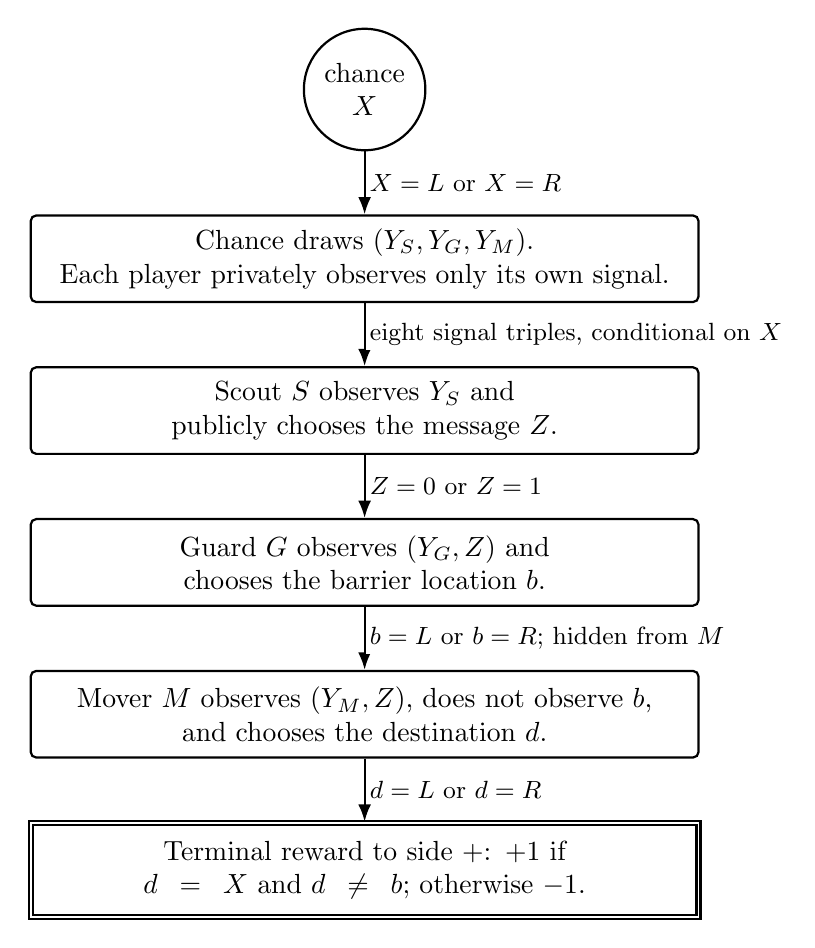
\begin{tikzpicture}[
    node distance=8mm,
    chance/.style={
      circle,
      draw,
      thick,
      minimum size=13mm,
      align=center
    },
    stage/.style={
      rectangle,
      rounded corners=2pt,
      draw,
      thick,
      text width=8.2cm,
      minimum height=11mm,
      align=center,
      inner sep=4pt
    },
    terminal/.style={
      rectangle,
      draw,
      double,
      thick,
      text width=8.2cm,
      minimum height=12mm,
      align=center,
      inner sep=4pt
    },
    flow/.style={-{Latex[length=2.2mm]},thick},
    branch/.style={font=\small,align=left,fill=white,inner sep=1.5pt}
]
\node[chance] (target) {chance\\$X$};
\node[stage, below=of target] (signals)
  {Chance draws $(Y_S,Y_G,Y_M)$.\\Each player privately observes only its own signal.};
\node[stage, below=of signals] (scout)
  {Scout $S$ observes $Y_S$ and\\publicly chooses the message $Z$.};
\node[stage, below=of scout] (guard)
  {Guard $G$ observes $(Y_G,Z)$ and\\chooses the barrier location $b$.};
\node[stage, below=of guard] (mover)
  {Mover $M$ observes $(Y_M,Z)$, does not observe $b$,\\and chooses the destination $d$.};
\node[terminal, below=of mover] (reward)
  {Terminal reward to side $+$: $+1$ if\\$d=X$ and $d\neq b$; otherwise $-1$.};

\draw[flow] (target) -- node[branch,right] {$X=L$ or $X=R$} (signals);
\draw[flow] (signals) -- node[branch,right] {eight signal triples, conditional on $X$} (scout);
\draw[flow] (scout) -- node[branch,right] {$Z=0$ or $Z=1$} (guard);
\draw[flow] (guard) -- node[branch,right] {$b=L$ or $b=R$; hidden from $M$} (mover);
\draw[flow] (mover) -- node[branch,right] {$d=L$ or $d=R$} (reward);
\end{tikzpicture}
\caption{Collapsed extensive-form tree for the hidden-location signaling game. Expanding every labeled branch produces the full tree. The boxes state the information available when each player acts.}
\label{fig:hidden-location-tree}
\end{figure}

The complete tree has $2\cdot2^3\cdot2^3=128$ terminal histories: two target values, eight signal triples, and eight subsequent action triples $(Z,b,d)$. Drawing all $128$ leaves in one picture would obscure the structure. Figures~\ref{fig:hidden-location-signal-tree} and~\ref{fig:hidden-location-action-tree} therefore split the expansion into two parts. Figure~\ref{fig:hidden-location-signal-tree} expands all chance outcomes. A copy of the decision subtree in Figure~\ref{fig:hidden-location-action-tree} is attached to each of its $16$ leaves.

\begin{figure}[p]
\centering
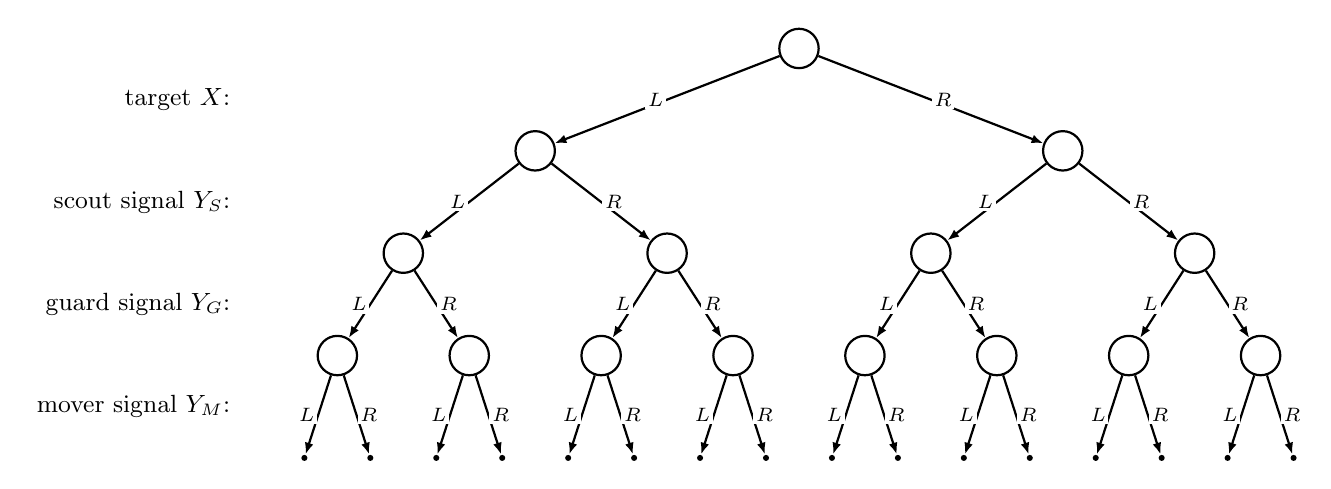
\begin{tikzpicture}[
    level distance=13mm,
    level 1/.style={sibling distance=67mm},
    level 2/.style={sibling distance=33.5mm},
    level 3/.style={sibling distance=16.75mm},
    level 4/.style={sibling distance=8.375mm},
    chance/.style={circle,draw,thick,minimum size=5mm,inner sep=0pt},
    leaf/.style={circle,fill=black,minimum size=2.2pt,inner sep=0pt},
    edge from parent/.style={draw,thick,-{Latex[length=1.5mm]}},
    value/.style={font=\scriptsize,fill=white,inner sep=1pt}
]
\node[chance] {}
child { node[chance] {}
  child { node[chance] {}
    child { node[chance] {}
      child { node[leaf] {} edge from parent node[value,left] {$L$} }
      child { node[leaf] {} edge from parent node[value,right] {$R$} }
      edge from parent node[value,left] {$L$}
    }
    child { node[chance] {}
      child { node[leaf] {} edge from parent node[value,left] {$L$} }
      child { node[leaf] {} edge from parent node[value,right] {$R$} }
      edge from parent node[value,right] {$R$}
    }
    edge from parent node[value,left] {$L$}
  }
  child { node[chance] {}
    child { node[chance] {}
      child { node[leaf] {} edge from parent node[value,left] {$L$} }
      child { node[leaf] {} edge from parent node[value,right] {$R$} }
      edge from parent node[value,left] {$L$}
    }
    child { node[chance] {}
      child { node[leaf] {} edge from parent node[value,left] {$L$} }
      child { node[leaf] {} edge from parent node[value,right] {$R$} }
      edge from parent node[value,right] {$R$}
    }
    edge from parent node[value,right] {$R$}
  }
  edge from parent node[value,left] {$L$}
}
child { node[chance] {}
  child { node[chance] {}
    child { node[chance] {}
      child { node[leaf] {} edge from parent node[value,left] {$L$} }
      child { node[leaf] {} edge from parent node[value,right] {$R$} }
      edge from parent node[value,left] {$L$}
    }
    child { node[chance] {}
      child { node[leaf] {} edge from parent node[value,left] {$L$} }
      child { node[leaf] {} edge from parent node[value,right] {$R$} }
      edge from parent node[value,right] {$R$}
    }
    edge from parent node[value,left] {$L$}
  }
  child { node[chance] {}
    child { node[chance] {}
      child { node[leaf] {} edge from parent node[value,left] {$L$} }
      child { node[leaf] {} edge from parent node[value,right] {$R$} }
      edge from parent node[value,left] {$L$}
    }
    child { node[chance] {}
      child { node[leaf] {} edge from parent node[value,left] {$L$} }
      child { node[leaf] {} edge from parent node[value,right] {$R$} }
      edge from parent node[value,right] {$R$}
    }
    edge from parent node[value,right] {$R$}
  }
  edge from parent node[value,right] {$R$}
};

\node[anchor=east,font=\small] at (-7.1,-0.65) {target $X$:};
\node[anchor=east,font=\small] at (-7.1,-1.95) {scout signal $Y_S$:};
\node[anchor=east,font=\small] at (-7.1,-3.25) {guard signal $Y_G$:};
\node[anchor=east,font=\small] at (-7.1,-4.55) {mover signal $Y_M$:};
\end{tikzpicture}
\caption{Expanded chance-and-signal part of the game tree. Reading the four edge labels along any root-to-leaf path gives one outcome $(X,Y_S,Y_G,Y_M)$. The $16$ leaves represent all target and signal combinations.}
\label{fig:hidden-location-signal-tree}
\end{figure}

\begin{figure}[p]
\centering
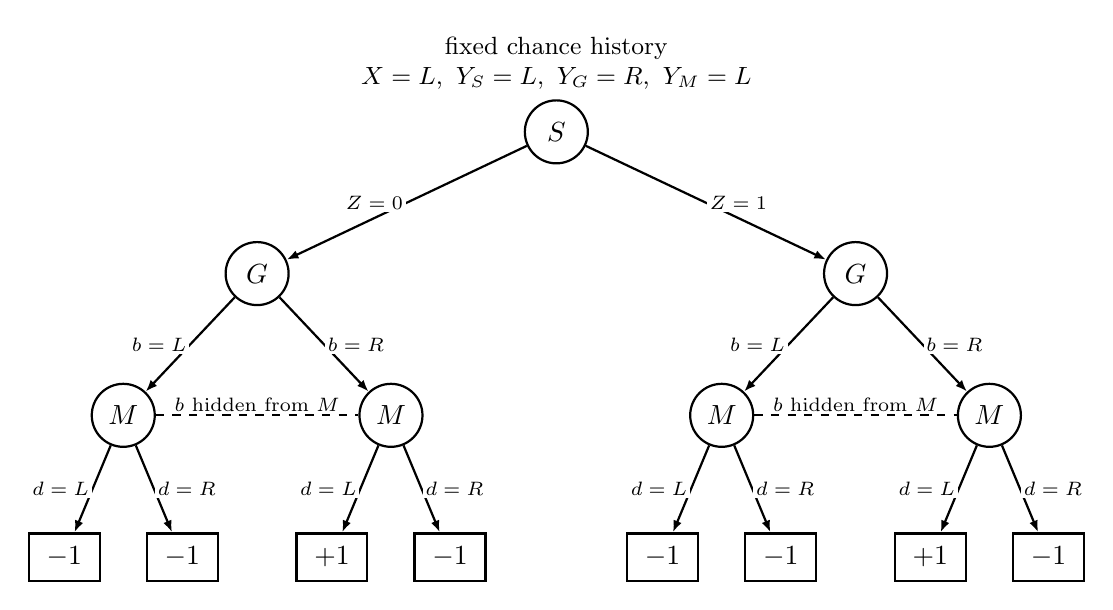
\begin{tikzpicture}[
    level distance=18mm,
    level 1/.style={sibling distance=76mm},
    level 2/.style={sibling distance=34mm},
    level 3/.style={sibling distance=15mm},
    decision/.style={circle,draw,thick,minimum size=8mm,inner sep=0pt},
    payoff/.style={rectangle,draw,thick,minimum width=9mm,minimum height=6mm,inner sep=1pt},
    edge from parent/.style={draw,thick,-{Latex[length=1.5mm]}},
    value/.style={font=\scriptsize,fill=white,inner sep=1pt},
    infoset/.style={dashed,thick}
]
\node[decision] (scoutnode) {$S$}
child { node[decision] (guardzero) {$G$}
  child { node[decision] (moverzerol) {$M$}
    child { node[payoff] {$-1$} edge from parent node[value,left] {$d=L$} }
    child { node[payoff] {$-1$} edge from parent node[value,right] {$d=R$} }
    edge from parent node[value,left] {$b=L$}
  }
  child { node[decision] (moverzeror) {$M$}
    child { node[payoff] {$+1$} edge from parent node[value,left] {$d=L$} }
    child { node[payoff] {$-1$} edge from parent node[value,right] {$d=R$} }
    edge from parent node[value,right] {$b=R$}
  }
  edge from parent node[value,left] {$Z=0$}
}
child { node[decision] (guardone) {$G$}
  child { node[decision] (moveronel) {$M$}
    child { node[payoff] {$-1$} edge from parent node[value,left] {$d=L$} }
    child { node[payoff] {$-1$} edge from parent node[value,right] {$d=R$} }
    edge from parent node[value,left] {$b=L$}
  }
  child { node[decision] (moveroner) {$M$}
    child { node[payoff] {$+1$} edge from parent node[value,left] {$d=L$} }
    child { node[payoff] {$-1$} edge from parent node[value,right] {$d=R$} }
    edge from parent node[value,right] {$b=R$}
  }
  edge from parent node[value,right] {$Z=1$}
};

\draw[infoset] (moverzerol) -- node[value,above] {$b$ hidden from $M$} (moverzeror);
\draw[infoset] (moveronel) -- node[value,above] {$b$ hidden from $M$} (moveroner);
\node[anchor=south,font=\small,align=center] at (scoutnode.north)
  {fixed chance history\\$X=L,\ Y_S=L,\ Y_G=R,\ Y_M=L$};
\end{tikzpicture}
\caption{Expanded action subtree attached to one leaf of Figure~\ref{fig:hidden-location-signal-tree}. The dashed lines join mover nodes that belong to the same information set because the mover observes $Z$ but not the guard's barrier $b$. For the displayed chance history, reward $+1$ occurs only when $b=R$ and $d=L=X$.}
\label{fig:hidden-location-action-tree}
\end{figure}

\clearpage

The figures make the three benefits concrete. For Challenge~1, Figure~\ref{fig:hidden-location-tree} displays the local decision cases: the scout acts from its signal, while the guard and mover act from a signal and the public message. A strategy representation can use these local decision points without listing the $64$ complete side-$+$ policies as separate matrix rows. For Challenge~2, every root-to-leaf path through Figures~\ref{fig:hidden-location-signal-tree} and~\ref{fig:hidden-location-action-tree} identifies one outcome and its probability, so the expected reward is the sum of terminal rewards weighted by their path probabilities. The tree organizes that calculation but does not remove its computational cost. For Challenge~3, the dashed lines in Figure~\ref{fig:hidden-location-action-tree} join histories that the mover cannot distinguish because it does not observe $b$. Requiring one action distribution for each dashed information set prevents the solver from using the hidden barrier. Similar information sets, omitted from the picture for readability, connect nodes across chance histories whenever the acting player has the same local history. Challenge~4 remains: the tree alone does not specify correlation between the scout's and mover's random choices, so Subsection~\ref{app:decentralized-teams} introduces additional team-strategy structure.

The tree describes all possible plays. To solve the game, one must next represent how players choose actions at its information sets. A \emph{pure contingent plan} for a player assigns one action to every information set of that player, including information sets that may not be reached. It is the extensive-form version of the complete local policy defined in Subsection~\ref{app:partially-observed-games}. A mixed strategy, as defined for one-stage games, is now a probability distribution over these complete pure contingent plans. A \emph{behavioral strategy} instead assigns a probability distribution over actions separately at each information set. Behavioral strategies expose the local choices shown by the tree and avoid explicitly sampling an entire pure plan whenever local randomization is sufficient.

Whether local randomization is sufficient depends on memory. A player has \emph{perfect recall} if, whenever it acts, its current local history retains all information it previously observed and all actions it previously chose. Two strategies are \emph{realization-equivalent} if, against every fixed profile of the other players, they induce the same probability distribution over terminal histories. In a finite perfect-recall game, every mixed strategy has a realization-equivalent behavioral strategy and conversely. This result permits complete-plan randomization to be replaced by local action probabilities without changing the distribution of outcomes. The equivalence can fail when a player has \emph{imperfect recall}, meaning that some earlier information or action is absent from its later local history.

Expected utilities and several game-solving algorithms require the probability of arriving at each node. For a strategy profile $\pi$, let $\operatorname{reach}_\pi(h)$ denote the \emph{reach probability}, the probability of history $h$. It can be factored as
\[
    \operatorname{reach}_\pi(h)
    =
    \operatorname{reach}_{i,\pi}(h)
    \operatorname{reach}_{-i,\pi}(h),
\]
where $\operatorname{reach}_{i,\pi}(h)$ is the product of player $i$'s action probabilities along $h$, and $\operatorname{reach}_{-i,\pi}(h)$ is the product of the probabilities contributed by chance and all other players. Multiplying a terminal history's reach probability by its utility and summing over terminal histories gives expected utility. Separating the acting player's contribution from the remaining contribution is also used by the counterfactual calculations introduced in Subsection~\ref{app:regret-cfr}.

The payoff matrices used in the hidden-location examples are normal-form representations. The \emph{normal form} converts an extensive-form game into a one-stage game by treating each complete pure contingent plan as one pure action. It therefore allows the matrix-game methods from Subsection~\ref{app:one-stage-equilibrium} to be applied, but the number of matrix rows and columns is usually enormous because every plan must specify an action at every information set.

The \emph{sequence form} retains the tree's local structure and gives a more compact representation for perfect-recall games. A player's \emph{action sequence} $\upsilon$ is the ordered list of that player's own actions along a path from the start of the game. The empty sequence is denoted by $\varnothing$. For information set $I$, let $\upsilon(I)$ be the player's action sequence before reaching $I$. Appending action $a\in A(I)$ produces the sequence $\upsilon(I)a$.

A \emph{realization weight} $x(\upsilon)$ is the probability contribution of the player's own strategy to sequence $\upsilon$. These weights satisfy the flow constraints
\[
    \sum_{a\in A(I)}x(\upsilon(I)a)=x(\upsilon(I)),
    \qquad
    x(\varnothing)=1,
    \qquad
    x(\upsilon)\geq0.
\]
The first equality distributes the weight arriving at an information set among its available actions. A collection of weights satisfying these constraints is called a \emph{realization plan}. Its size is proportional to the number of action sequences rather than the number of complete pure plans, although it can still be large when the underlying tree is large.

The benefit of this representation is that the realization-plan constraints are linear. Every linear program has an associated \emph{dual program}. Feasible solutions of one program provide bounds on the objective of the other, and under the usual feasibility conditions their optimal objective values are equal.

For a finite two-player zero-sum perfect-recall game, the expected payoff can be written
\[
    u(x,y)=x^{\mathsf T}M_{\mathrm{seq}}y,
\]
where $x$ and $y$ are the two players' realization plans and the matrix $M_{\mathrm{seq}}$ records terminal utilities and chance probabilities. The equilibrium problem can then be expressed through a pair of dual linear programs whose bounds agree at an exact solution \cite{koller1996sequence}. Thus, for this class of games, the tree makes it possible to solve from local action sequences without first constructing the much larger matrix of complete pure plans.

This linear-program conclusion does not apply directly to every game represented by a tree. In particular, the scout and mover in the hidden-location examples are separate teammates. If they randomize independently, the probability of a scout--mover policy pair must factor into the product of their separate probabilities. These product constraints are exactly what made the independent-randomization problems in Subsections~\ref{app:partially-observed-games} and~\ref{app:repeated-hidden-location} bilinear and nonconvex. If shared randomization over complete scout--mover plans is allowed, the resulting two-side normal-form game can instead be solved by a linear program, but the number of complete plans may be enormous. The tree remains useful in either case because it records the local decisions and information restrictions, even when it does not produce a linear optimization problem.

Sequence form avoids normal-form policy enumeration, but it does not remove the large number of histories in a game such as bridge. This remaining growth motivates approximate representations. An \emph{abstraction} replaces a large set of states, histories, information sets, actions, or private types by a smaller representation. It is \emph{lossless} if solving the reduced game preserves the original game value and optimal strategies. Otherwise the difference introduced by the reduction is called \emph{abstraction error}. \emph{Function approximation} represents a large table of policy or value entries by a function $f_\theta$ determined by a smaller parameter vector $\theta$.


\subsection{Bridge bidding as an instance of the framework}

Contract bridge has four players
\[
    \{S,W,N,E\},
\]
with partnerships $\{S,N\}$ and $\{E,W\}$. Chance deals thirteen cards to each player. A player's hand is private information. The auction is a public sequence of calls, and the acting seat rotates in fixed order. A legal call is an action. The complete deal, public auction, dealer, vulnerability, and seat to act form a Markov state for the mathematical model. Each player observes only its own hand and the public components of this state.

The hidden deal is sampled once and remains fixed during bidding. To embed the auction in the general POMG above, the seat-to-act component of the state designates the active player. At each call, that player chooses one legal bridge call, while the other three players have only a no-op action. State transitions after the deal are deterministic: the selected legal call is appended to the auction, the seat to act advances, and the no-op actions have no effect. The terminal reward is the raw bridge score assigned to the final contract and play outcome. Raw score means the ordinary numerical table score for the board before any comparison with another table or field.

In the extensive-form representation, a history contains the deal generated by chance and the calls made so far. Two histories belong to the same information set for a player when that player has the same hand and sees the same public auction in both histories. Each individual player has perfect recall. Naively merging both partners into one player can create imperfect recall because the merged player does not possess both private hands at each decision \cite{gimbert2020bridge}.


\subsection{Decentralized teams and correlation}
\label{app:decentralized-teams}

A team is a specified subset of players whose members have the same utility but may possess different private information and choose actions separately.

Let $\Pi_S,\Pi_N,\Pi_E,\Pi_W$ denote sets of pure local contingent plans. A pure South--North joint plan is
\[
    \varphi_{SN}=(\varphi_S,\varphi_N)\in\Pi_S\times\Pi_N.
\]
A correlated partnership strategy is a distribution
\[
    \lambda_{SN}\in\Delta(\Pi_S\times\Pi_N).
\]
The term \emph{ex ante} means before the random deal and hence before either partner receives private information. Ex ante, the partnership jointly samples $(\varphi_S,\varphi_N)$ from $\lambda_{SN}$. During the auction, South follows $\varphi_S$ using only South's information and North follows $\varphi_N$ using only North's information. The sampled plans may be statistically correlated even though the partners cannot exchange their private hands.

Independent randomization is more restrictive. Let
\[
    \lambda_S\in\Delta(\Pi_S),
    \qquad
    \lambda_N\in\Delta(\Pi_N)
\]
be separate distributions over South's and North's pure plans. Their joint distribution then has the product form
\[
    \lambda_{SN}(\varphi_S,\varphi_N)
    =
    \lambda_S(\varphi_S)\lambda_N(\varphi_N),
\]
or, at the behavioral level, independent random choices at local information sets. A general correlated strategy need not factor this way.

Let $\Lambda_{SN}$ and $\Lambda_{EW}$ be the allowed sets of correlated partnership strategies, and let
\[
    U(\lambda_{SN},\lambda_{EW})
\]
be expected South--North raw score. A correlated team max--min equilibrium is a saddle point of
\[
    \max_{\lambda_{SN}\in\Lambda_{SN}}
    \min_{\lambda_{EW}\in\Lambda_{EW}}
    U(\lambda_{SN},\lambda_{EW}).
\]
In the adversarial-team literature, TMECor abbreviates \emph{team-maxmin equilibrium with correlation}: a team max--min equilibrium that permits ex-ante correlation over joint plans \cite{farina2018coordination,farina2021collusion}.

A partnership best response must optimize both local plans jointly:
\[
    \operatorname{BR}_{SN}(\lambda_{EW})
    \in
    \arg\max_{\lambda_{SN}\in\Lambda_{SN}}
    U(\lambda_{SN},\lambda_{EW}).
\]
Updating South while holding North fixed computes only a unilateral response and may miss improvements requiring both partners to change the meaning of calls.

Common information is information observed by all members of the relevant team, such as the public auction. Private information is observed by only one member, such as a hand. For team member $i$, let $\Xi_i$ be the set of possible private-information values and let $\xi_{i,t}\in\Xi_i$ be the value actually held by that member at time $t$. Together, $(\chi_t,\xi_{i,t})$ determine player $i$'s local history $h_{i,t}$.

A \emph{prescription} for player $i$ is a function
\[
    \gamma_{i,t}(\cdot\mid\chi_t,\xi_{i,t})
    \in
    \Delta(A_{i,t}(h_{i,t}))
\]
that assigns a legal action distribution to every possible private-information value. A \emph{coordinator} is a representation device, not an additional player with access to all private information. It observes only the team's common information $\chi_t$ and chooses one prescription for each team member. The real player $i$ then applies the selected prescription to its own realized value $\xi_i$. PublicTeamConversion replaces the decentralized team by this common-information coordinator and its prescriptions, preserving the original information restrictions while making the team's joint choice explicit \cite{carminati2022marriage}.

Let $\mathcal{J}$ denote the set of players in the team and let
\[
    \xi_{\mathcal{J},t}=(\xi_{i,t})_{i\in\mathcal{J}}
\]
be the vector of their private-information values at time $t$. Let $\chi_t$ be the common information available at time $t$, including previous prescriptions when they affect the distribution. A \emph{common-information belief} applies the belief definition above to the hidden pair $(s_t,\xi_{\mathcal{J},t})$ and the observed common information $\chi_t$. The conditional probability of $(s,\xi_{\mathcal{J}})$ is denoted by $\beta_t^{\mathrm{com}}(s,\xi_{\mathcal{J}}\mid\chi_t)$. A common-information-belief dynamic program uses the pair $(\chi_t,\beta_t^{\mathrm{com}}(\cdot,\cdot\mid\chi_t))$ as the state of a centralized planning problem \cite{kartik2022competingteams}.

A \emph{directed graph} consists of nodes connected by directed edges. It is \emph{acyclic} if no sequence of directed edges returns to its starting node. A directed acyclic graph is abbreviated DAG. The \emph{Team Belief DAG} organizes common-information states, private-information possibilities, and feasible correlated realization weights in such a graph. Its linear flow constraints extend the sequence-form realization-plan constraints to decentralized teams and allow optimization over correlated team strategies within the represented strategy class \cite{zhang2023teambelief}. Guarantees from this construction require that the game and its information structure satisfy the assumptions of the representation; they do not automatically apply to an arbitrary team game.


\subsection{Exact solutions, approximations, and diagnostics}
\label{app:exact-approximations}

A solution concept specifies the mathematical target: examples are a best response, saddle point, Nash equilibrium, or TMECor. An algorithm is a procedure intended to compute that target.

An \emph{exact algorithm} returns a strategy satisfying the chosen solution concept for the stated finite model, apart from numerical roundoff in computer arithmetic. An \emph{approximate algorithm} returns a candidate strategy without proving that it exactly satisfies the solution concept. A \emph{certified approximation} also returns a mathematically valid error bound, such as an exploitability gap no larger than $\epsilon$. When a small abstraction can be solved exactly, its exact solution is often called \emph{ground truth} because it provides a reference against which approximate methods can be tested.

\subsubsection{Example: Nash equilibrium without a saddle point}
\label{app:nash-without-saddle}

Consider a two-player coordination game in which each player chooses either $A$ or $B$. Both players receive utility $1$ when their actions agree and utility $0$ when they differ:
\[
    \begin{array}{c|cc}
        & A & B\\ \hline
        A & (1,1) & (0,0)\\
        B & (0,0) & (1,1)
    \end{array}.
\]
The profiles $(A,A)$ and $(B,B)$ are Nash equilibria because either player would reduce its utility by deviating alone. They are not saddle points. For example, if the common payoff is written as
\[
    M=
    \begin{pmatrix}
        1&0\\
        0&1
    \end{pmatrix},
\]
the saddle-point inequality fails at $(A,A)$ because its right-hand inequality would require
\[
    u(A,A)\leq u(A,B),
\]
whereas $u(A,A)=1$ and $u(A,B)=0$. The reason is that the second player maximizes the same payoff rather than minimizing it.

A \emph{self-play evaluation} measures the expected payoff when the participating strategies are produced by the same learning procedure. A \emph{fixed-benchmark score} is the expected payoff against one opponent strategy that is held unchanged throughout evaluation. \emph{Cross-play} evaluates many strategy pairs drawn from a set of independently trained or historical strategies and records the resulting payoffs in a matrix. None of these measurements alone is an equilibrium certificate because none necessarily evaluates a best response.

An \emph{exact best-response solver} finds a true best response within the stated strategy space and can therefore be used to compute the exploitability gap. An \emph{approximate best-response solver} searches for an improving response but may fail to find the best one. Any improvement it discovers is then only a lower bound on true exploitability. Failure to discover a stronger response does not prove that no stronger response exists.


\subsection{Regret minimization and CFR}
\label{app:regret-cfr}

Consider a sequence of $T$ optimization rounds. Let $X\subseteq\mathbb{R}^d$ be the set of available decision vectors. At round $t$, the decision maker selects $x_t\in X$. After that selection, a payoff vector $g_t\in\mathbb{R}^d$ is revealed, and the round payoff is the inner product $g_t\cdot x_t$.

The \emph{external regret} after $T$ rounds compares the accumulated payoff of the selected sequence with the accumulated payoff that would have been obtained by using the best single fixed decision $x\in X$ on every round:
\[
    R_T
    =
    \max_{x\in X}
    \sum_{t=1}^T g_t\cdot x
    -
    \sum_{t=1}^T g_t\cdot x_t.
\]
An algorithm is \emph{no-regret} if its average regret satisfies $R_T/T\to0$ as $T\to\infty$. If both players in a finite two-player zero-sum game repeatedly update their strategies using no-regret algorithms, the averages of their played strategies approach the set of equilibria.

\emph{Counterfactual regret minimization} (CFR) applies regret minimization separately at each information set. Its values are called \emph{counterfactual} because, when evaluating an information set, the calculation weights histories by the reach probabilities contributed by chance and the other players while omitting player $i$'s own probability of reaching that information set.

Let $ha$ denote the history obtained by appending action $a$ to history $h$. Let $c_\pi(z\mid ha)$ be the probability of terminal history $z$ when play continues from $ha$ according to strategy profile $\pi$. For player $i$, information set $I$, and action $a$, define the counterfactual action value
\[
    v_i^\pi(I,a)
    =
    \sum_{h\in I}
    \operatorname{reach}_{-i,\pi}(h)
    \sum_{z\succeq ha}
    c_\pi(z\mid ha)u_i(z),
\]
where $z\succeq ha$ means that terminal history $z$ extends history $ha$. The value under the current action distribution is
\[
    v_i^\pi(I)
    =
    \sum_{a\in A(I)}
    \pi_i(a\mid I)v_i^\pi(I,a).
\]
At iteration $t$, the \emph{instantaneous counterfactual regret} for action $a$ is the difference between the value of always selecting $a$ at $I$ and the value of the current action distribution:
\[
    \operatorname{reg}_t(I,a)
    =
    v_i^{\pi_t}(I,a)-v_i^{\pi_t}(I).
\]
The \emph{cumulative counterfactual regret} is
\[
    R_T(I,a)=\sum_{t=1}^T \operatorname{reg}_t(I,a).
\]
\emph{Regret matching} constructs the next action distribution from the positive parts of these cumulative regrets:
\[
    \pi_{i,T+1}(a\mid I)
    =
    \frac{[R_T(I,a)]_+}
         {\sum_{a'}[R_T(I,a')]_+},
\]
when the denominator is positive, where $[x]_+=\max\{x,0\}$. If all positive regrets are zero, a fixed fallback distribution, commonly the uniform distribution, is used. In two-player zero-sum perfect-recall games, the reach-weighted average strategy produced by CFR approaches equilibrium as average regret decreases \cite{zinkevich2007regret}.

A \emph{team-aware CFR} method first represents each partnership by a valid convex set of correlated team strategies, such as the coordinator or Team Belief DAG constructions, and then applies regret minimization to that representation. Its equilibrium guarantee requires the assumptions of the chosen convex representation and the corresponding perfect-recall-style information structure; applying ordinary CFR directly to separate bridge teammates does not establish that guarantee.


\subsection{Supervised learning and representation learning}

A \emph{training example} is a pair $(x_k,y_k)$ consisting of an input $x_k$ and a desired output or \emph{target} $y_k$. Let $N_{\mathrm{train}}$ be the positive integer giving the number of examples. A \emph{training data set} is the finite collection
\[
    \mathcal{T}_{\mathrm{data}}=\{(x_k,y_k)\}_{k=1}^{N_{\mathrm{train}}}.
\]
A \emph{parameterized predictor} is a function $f_\theta$ whose behavior is determined by a parameter vector $\theta$. A \emph{loss function} $\ell(\widehat y,y)$ assigns a numerical penalty when prediction $\widehat y$ is compared with target $y$.

\emph{Supervised learning} chooses the parameters to minimize the average loss on the training data. The \emph{empirical loss} is
\[
    \widehat L(\theta)
    =
    \frac{1}{N_{\mathrm{train}}}
    \sum_{k=1}^{N_{\mathrm{train}}}
    \ell(f_\theta(x_k),y_k).
\]
Training seeks a parameter value in $\arg\min_{\theta\in\Theta}\widehat L(\theta)$.

A \emph{classification problem} has targets drawn from a finite set of labels. When the labels are actions and $\pi_\theta(\cdot\mid x_k)$ is a predicted probability distribution over them, the \emph{cross-entropy loss} for example $k$ is
\[
    \ell_k(\theta)
    =
    -\log\pi_\theta(y_k\mid x_k).
\]
\emph{Imitation learning} is supervised learning in which the target actions are generated by a human, a program, or another policy. \emph{Supervised pretraining} first fits such targets and then uses the resulting parameters as the starting point for a later learning procedure based on interaction.

\emph{Cost-sensitive classification} assigns different losses to different kinds of classification error rather than treating every incorrect label equally. \emph{Co-training} alternates between two or more predictors, using predictions from one predictor to construct or refine training information for another.

A \emph{neural network} is a parameterized function formed by composing affine transformations with nonlinear componentwise functions. A network with several intermediate, or hidden, layers is commonly called a \emph{deep neural network}. A \emph{belief network} $b_\phi$ is a parameterized predictor whose output is a probability distribution over hidden variables.

A \emph{primary loss} measures the main prediction or decision objective. An \emph{auxiliary loss} measures an additional desired property. They may be combined as
\[
    L_{\mathrm{total}}(\theta,\phi)
    =
    L_{\mathrm{primary}}(\theta)
    +
    \lambda_{\mathrm{aux}} L_{\mathrm{aux}}(\theta,\phi),
\]
where $\lambda_{\mathrm{aux}}\geq0$ controls the weight of the auxiliary term. For bridge, an auxiliary loss may encourage accurate prediction of hidden hands.

\emph{Representation learning} trains a parameterized map that converts an input into a feature vector useful for later prediction or decision making. Such a map is called an \emph{embedding}. If $X$ is the input space and $d_{\mathrm{emb}}$ is the feature dimension, an embedding has the form
\[
    e_\psi:X\to\mathbb{R}^{d_{\mathrm{emb}}}.
\]
A \emph{recurrent history encoder} maintains a memory vector $m_t$ and updates it after each new observation and action:
\[
    m_t=F_\psi(m_{t-1},o_t,a_{t-1})
\].
The same update function $F_\psi$ is reused at every time. The resulting memory vector is a learned summary of the local history.

\emph{Parameter sharing} means that several players use the same parameter vector while player-specific information, such as seat or partnership orientation, is supplied as input. \emph{Data augmentation} creates additional training examples by applying transformations known to preserve the task, such as consistent suit permutations. \emph{Legal-action masking} sets the predicted probability of every illegal action to zero and renormalizes the remaining probabilities.

\emph{Deep CFR} uses deep neural networks to approximate counterfactual regrets and average strategies instead of storing a separate table entry for every information set \cite{brown2019deep}.


\subsection{Reinforcement learning and PPO}
\label{app:reinforcement-learning}

In reinforcement-learning terminology, an \emph{agent} is the decision maker together with its policy and any procedure used to update that policy. The \emph{environment} is the sequential decision system with which the agent interacts, including its states, legal actions, transitions, and rewards. \emph{Reinforcement learning} updates values or policies using trajectories generated through this interaction rather than using a data set of labeled optimal actions. A \emph{discount factor} is a number $\gamma\in[0,1]$ that reduces the weight assigned to rewards received further in the future. The \emph{discounted return} from time $t$ is
\[
    G_t
    =
    \sum_{k=t}^{H-1}
    \gamma^{k-t}r_k(s_k,a_k,s_{k+1}).
\]
For finite-horizon bridge bidding with terminal score, $\gamma=1$ is natural because there is no reason to value the terminal score less merely because the auction was longer.

A \emph{model-free method} learns values or policies without first constructing an explicit model of transition or observation probabilities. A \emph{model-based method} uses a known or learned model of transitions, observations, or other players' behavior to predict future events, plan, or simulate trajectories.

For a local history $h_t$, the \emph{history-based action-value function} under policy $\pi$ is
\[
    Q_t^\pi(h_t,a)
    =
    \mathbb{E}
    \left[
      G_t
      \mid h_t,a_t=a
    \right],
\]
where the expectation uses the trajectory distribution generated by policy $\pi$. The history-based value is
\[
    V_t^\pi(h_t)
    =
    \sum_a
    \pi(a\mid h_t)Q_t^\pi(h_t,a).
\]
The second equation averages the action values using the probabilities assigned by the current policy.

\emph{Q-learning} stores or approximates an action-value function and updates it after an observed transition. In a fully observed MDP, the current state replaces the local history, so the action-value estimate is written as $Q(s,a)$. One update is
\[
    Q(s_t,a_t)
    \leftarrow
    Q(s_t,a_t)
    +
    \alpha
    \left[
      r_t(s_t,a_t,s_{t+1})
      +
      \gamma\max_{a'}Q(s_{t+1},a')
      -
      Q(s_t,a_t)
    \right]
\]
\cite{watkins1992qlearning}. Here $\alpha\in(0,1]$ is the learning rate controlling the size of the update. The quantity
\[
    r_t(s_t,a_t,s_{t+1})+\gamma\max_{a'}Q(s_{t+1},a')
\]
is the \emph{one-step target}: the observed immediate reward plus the estimated optimal continuation value from the next state. The expression inside square brackets is the target minus the current estimate. The standard convergence results for tabular Q-learning require a fully observed Markov state, sufficient exploration, and appropriate learning-rate conditions. Under partial observation, a full local history or a sufficient statistic such as a belief state can replace the state argument. A learned recurrent representation is commonly used as a heuristic, but it need not be Markov or sufficient and therefore does not inherit the tabular Q-learning guarantee. \emph{Penetrative Q-learning} is a bridge-specific modification that propagates terminal auction evaluations through additional earlier auction decisions \cite{yeh2016automatic}.

For a parameterized policy $\pi_\theta$, define
\[
    J(\theta)=J(\pi_\theta).
\]
A \emph{policy-gradient method} adjusts $\theta$ in a direction that increases this expected return. The \emph{advantage}
\[
    A_t
    =
    Q_t^\pi(h_t,a_t)-V_t^\pi(h_t)
\]
measures how much better the selected action is than the policy's average action at the same history. Let $\widehat A_t$ denote an estimate of $A_t$. The \emph{likelihood-ratio identity} rewrites the derivative of a probability-weighted expectation using derivatives of log probabilities. Applied to a policy, it gives the schematic gradient
\[
    \nabla_\theta J(\theta)
    =
    \mathbb{E}
    \left[
      \sum_t
      \nabla_\theta
      \log\pi_\theta(a_t\mid h_t)
      A_t
    \right],
\]
where the expectation is over trajectories generated by the current policy \cite{sutton2000policygradient}.

\emph{Proximal Policy Optimization} (PPO) uses a clipped surrogate objective to discourage overly large improvements in sampled action-probability ratios during one update. It does not guarantee that every action probability or ratio remains within the clipping interval. Let $\theta_{\mathrm{old}}$ denote the parameters used to generate the sampled trajectories. The probability ratio for sampled action $a_t$ is
\[
    \rho_t(\theta)
    =
    \frac{\pi_\theta(a_t\mid h_t)}
         {\pi_{\theta_{\mathrm{old}}}(a_t\mid h_t)}.
\]
For a clipping parameter $\epsilon_{\mathrm{clip}}>0$, PPO maximizes the following objective, whose expectation is over sampled time steps from trajectories generated by $\pi_{\theta_{\mathrm{old}}}$:
\[
    L^{\mathrm{clip}}(\theta)
    =
    \mathbb{E}
    \left[
      \min
      \left(
        \rho_t(\theta)\widehat A_t,
        \operatorname{clip}
        (\rho_t(\theta),1-\epsilon_{\mathrm{clip}},1+\epsilon_{\mathrm{clip}})
        \widehat A_t
      \right)
    \right]
\]
\cite{schulman2017ppo}.
The clipping function
\[
    \operatorname{clip}(x,\ell,u)
    =
    \min\{u,\max\{\ell,x\}\}
\]
limits $x$ to the interval $[\ell,u]$.

The \emph{entropy} of an action distribution is
\[
    \operatorname{Ent}(\pi(\cdot\mid h))
    =
    -\sum_a\pi(a\mid h)\log\pi(a\mid h).
\]
\emph{Entropy regularization} adds a weighted entropy term to the training objective, encouraging the policy to retain nonzero probability on several actions during learning. \emph{Diverse PPO} trains several PPO variants with different clipping or entropy settings and combines them to reduce dependence on one locally optimal policy \cite{zhang2025diverse}.


\subsection{Self-play and coordinated policy improvement}
\label{app:self-play}

A \emph{learning system} is the complete procedure that generates data, updates policies, and stores any intermediate models. \emph{Self-play} generates training games in which the participating policies are produced by the same learning system. \emph{Latest-policy self-play} trains against the newest available opposing policies. A \emph{checkpoint} is a stored copy of a policy from an earlier training iteration. A \emph{policy population} is a finite collection of current or stored policies. \emph{Checkpoint self-play} samples opponents from a population of stored checkpoints. This broadens the set of encountered opponents and can reduce \emph{forgetting}, meaning loss of performance against policies that were handled successfully earlier in training.

An \emph{iterative policy-update procedure} is an algorithm that produces a sequence of policies
\[
    \pi^{(0)},\pi^{(1)},\pi^{(2)},\ldots,
\]
where the policy at iteration $t+1$ is computed using information obtained from policies and games available by iteration $t$. The procedure converges if the sequence approaches a limiting policy or limiting strategy profile. It cycles if it repeatedly returns to earlier policies or repeats the same pattern of policy changes instead of approaching a limit.

Non-transitivity is one possible cause of cycling. Suppose both sides of a two-player zero-sum game can use strategies from the same collection $\mathcal{Q}$. For $A,B\in\mathcal{Q}$, the game determines the expected utility
\[
    u(A,B)
\]
of the first side when it uses strategy $A$ against strategy $B$. Define
\[
    A\succ B
    \quad\Longleftrightarrow\quad
    u(A,B)>0.
\]
The relation $\succ$ is \emph{transitive} if
\[
    A\succ B
    \quad\text{and}\quad
    B\succ C
    \quad\Longrightarrow\quad
    A\succ C
\]
for every three strategies $A,B,C$. It is \emph{non-transitive} if this implication fails. A common form is the cycle
\[
    A\succ B,\qquad B\succ C,\qquad C\succ A.
\]
An update that trains only against the latest opponent may then move from a strategy like $A$ to one like $B$, then to $C$, and then back toward $A$. Training against a policy population reduces reliance on a single latest opponent.

\emph{Policy iteration} starts with a policy and alternates between two steps. The first step computes the value function of the current policy. The second step replaces the policy by one that chooses actions having the largest action values computed from that value function. In a finite fully observed MDP, exact policy evaluation and improvement terminate at an optimal policy. In a game with several players, a \emph{unilateral improvement} changes one player's policy while holding all other policies fixed; alternating such improvements need not converge and can cycle.

Let $\mathcal{J}=\{i_1,i_2\}$ be a two-player team, let $\pi_{-\mathcal{J}}$ denote the policies of players outside the team, and let $J_{\mathcal{J}}$ be the team's expected utility. Let $\Pi_{i_1}$ and $\Pi_{i_2}$ be the admissible policy classes for the two team members. \emph{Joint policy search} considers coordinated replacements $\pi'_{i_1}$ and $\pi'_{i_2}$ by solving or approximating
\[
    \max_{\substack{\pi'_{i_1}\in\Pi_{i_1}\\
                     \pi'_{i_2}\in\Pi_{i_2}}}
    J_{\mathcal{J}}(\pi'_{i_1},\pi'_{i_2},\pi_{-\mathcal{J}}).
\]
It can discover a new convention that requires both teammates to change simultaneously \cite{tian2020joint}.

\emph{Regularization} modifies an optimization objective to discourage undesirable changes or overly complex solutions. A \emph{divergence} $D(x\Vert x_0)$ is a nonnegative measure of discrepancy between strategy $x$ and a \emph{reference strategy} $x_0$, with $D(x\Vert x_0)=0$ when they are equal. Given reference strategies $(x_0,y_0)$ and regularization weight $\lambda_{\mathrm{reg}}>0$, one may solve
\[
    \max_x\min_y
    \left[
      u(x,y)
      -
      \lambda_{\mathrm{reg}}D(x\Vert x_0)
      +
      \lambda_{\mathrm{reg}}D(y\Vert y_0)
    \right].
\]
Here $x$ and $y$ range over the two players' allowed strategy sets; the first player maximizes the displayed quantity and the second player minimizes it.
\emph{Regularized Nash Dynamics} repeatedly updates both the strategies and their references while retaining an equilibrium of the original unregularized game as the target \cite{perolat2022deepnash}. A \emph{last-iterate guarantee} concerns the current strategy produced at iteration $t$. An \emph{average-iterate guarantee} concerns an average of strategies produced over many iterations; the average may converge even when the current strategies continue to oscillate.


\subsection{Fictitious play, double oracle, and PSRO}
\label{app:psro}

\emph{Fictitious play} repeatedly computes a best response to the uniform mixture of an opponent's previous strategies. If $y_1,\ldots,y_t$ are player 2's previous strategies, their \emph{empirical mixture} is
\[
    \bar y_t=\frac{1}{t}\sum_{k=1}^t y_k.
\]
The expression means that one of the previous strategies is selected uniformly at random. Player 1's next strategy is a best response, or an approximate best response, to $\bar y_t$. \emph{Fictitious self-play} applies this procedure using games generated by the learning system. \emph{Neural Fictitious Self-Play} uses reinforcement learning to approximate best responses and supervised learning to represent the empirical mixture \cite{heinrich2015fictitious,heinrich2016nfsp}.

A \emph{double-oracle algorithm} maintains a finite subset of each player's full strategy set. These subsets define a \emph{restricted game}. The algorithm computes an equilibrium of the restricted game, computes a best response in the full strategy space for each player, adds any new responses to the restricted sets, and repeats. If exact full-game best responses add no new strategy, the restricted-game equilibrium is also an equilibrium of the full finite game.

\emph{Policy-Space Response Oracles} (PSRO) generalizes this idea when responses are computed approximately. It maintains one policy population for each player:
\[
    \mathcal{Q}_1=\{\pi_1^1,\ldots,\pi_1^m\},
    \qquad
    \mathcal{Q}_2=\{\pi_2^1,\ldots,\pi_2^n\}.
\]
Let $J(\pi_1^j,\pi_2^k)$ denote the expected payoff to player 1 when those two policies are played. The \emph{empirical meta-game matrix} is
\[
    M_{jk}=J(\pi_1^j,\pi_2^k).
\]
A \emph{meta-solver} computes mixed strategies $(x,y)$ in this finite matrix game. To play mixture $y$, player 2 samples a policy index $k$ with probability $y_k$ and then uses policy $\pi_2^k$ for the complete episode. A \emph{response oracle} is an algorithm that attempts to construct a best response to such a mixture. For player 1, it approximately solves
\[
    \pi_1^{\mathrm{new}}
    \approx
    \operatorname{BR}_1
    (y),
\]
where $\operatorname{BR}_1(y)$ denotes a best response to the opponent population sampled according to $y$. PSRO adds the resulting policy to the population and repeats \cite{lanctot2017psro}.

\emph{Team-PSRO} stores joint team policies and uses reinforcement learning to approximate a coordinated team best response \cite{mcaleer2023teampsro}. \emph{Extensive-Form Double Oracle} and its neural approximation, Neural XDO, allow mixing at information sets rather than only sampling one complete policy before the game begins \cite{mcaleer2021xdo}.


\subsection{Monte Carlo evaluation and search}
\label{app:monte-carlo-search}

\emph{Monte Carlo estimation} approximates an expectation by averaging randomly generated samples. Let $N_{\mathrm{MC}}$ be a positive integer. If $X_1,\ldots,X_{N_{\mathrm{MC}}}$ are independent samples having the same distribution as random variable $X$, the Monte Carlo estimate is
\[
    \widehat{\mathbb{E}}[X]
    =
    \frac{1}{N_{\mathrm{MC}}}\sum_{k=1}^{N_{\mathrm{MC}}} X_k.
\]
\emph{Model-based Monte Carlo} generates the samples from a specified probabilistic model. In bridge, a sample may be a complete deal drawn from a belief distribution conditional on the acting player's hand and the public auction.

A \emph{determinization} is one sampled complete hidden state that is temporarily treated as if it were fully observed. Solving several determinizations independently can cause \emph{strategy fusion}: the calculation may select different future actions in hidden states that the real player cannot distinguish, even though one implementable policy must choose the same action whenever its information is the same.

A \emph{subtree} is the part of a tree consisting of one selected node and all of its descendants. \emph{Monte Carlo CFR} estimates the counterfactual-value sums used by CFR from randomly sampled histories or subtrees instead of traversing the complete game tree \cite{lanctot2009monte}.

An \emph{upper-confidence-bound} (UCB) rule balances exploitation of actions with high estimated value and exploration of actions having few samples. One common score is
\[
    \operatorname{UCB}(a)
    =
    \widehat\mu_a
    +
    c_{\mathrm{UCB}}\sqrt{\frac{\log N_{\mathrm{tot}}}{N_a}},
\]
where $\widehat\mu_a$ is the sample-mean value of action $a$, $N_a$ is the number of times action $a$ has been sampled, $N_{\mathrm{tot}}$ is the total number of action samples, and $c_{\mathrm{UCB}}>0$ controls the strength of exploration.
The displayed score is used after every candidate action has been sampled at least once; an implementation may instead assign an infinite score to an unvisited action.

\emph{Online search} performs additional computation when an action must actually be selected, rather than fixing every decision before the episode begins. A \emph{blueprint} is the complete policy available before this online computation. A \emph{partial policy} specifies actions only at the information sets considered inside one search. A \emph{search tree} represents possible future actions, observations, and successor histories from the current point. A node that is not expanded further is called a \emph{leaf}; its continuation value is supplied either by an exact terminal reward or by an approximate value function.

A \emph{public belief} uses the same belief concept but conditions only on the public history: it is the conditional probability distribution over hidden states and private information given that history. \emph{Belief Monte Carlo search} samples hidden states from this distribution and simulates continuations from those samples. \emph{Bayesian Action Decoder} is a cooperative search method that combines a public belief with sampled partial policies so that actions can be evaluated both for their immediate consequences and for the information they communicate \cite{foerster2019bad}.

A \emph{local search} changes the policy only in the continuation of the current public history. Such a change is \emph{unsafe} if it can increase exploitability because other information sets or earlier communicated meanings are ignored. The \emph{boundary} of the local continuation is the set of nodes at which the earlier game enters the part being solved locally. \emph{Continual resolving} repeatedly solves a local continuation game while retaining constraints on the values available to the opponent at this boundary \cite{burch2014solving}. ReBeL combines self-play, public-belief states, learned continuation values, and online search \cite{brown2020rebel}. SPARTA is a cooperative search method that accounts for what teammates can infer from deviations from the blueprint policy \cite{lerer2020sparta}.

A \emph{Bellman update} replaces a current value estimate by the immediate reward plus the estimated value of the next state, with the appropriate expectation and optimization over possible transitions and actions. \emph{Value iteration} starts with value estimates and repeatedly applies Bellman updates. Each update replaces the value of a state by the largest, over its legal actions, of the expected immediate reward plus the current estimate of the optimal value at the next state.

A \emph{statistic} is a function of the observed history; write $\sigma_t=f_t(h_t)$. The statistic is \emph{sufficient for future decision making} if any two histories $h_t$ and $\widetilde h_t$ satisfying $f_t(h_t)=f_t(\widetilde h_t)$ have the same legal actions and, for every such action, give both the same expected immediate reward and the same probability distribution for the next statistic $\sigma_{t+1}$. Consequently, the optimal continuation value and an optimal action depend on the history only through $\sigma_t$. In a stationary POMDP, the belief state satisfies the reward and next-statistic conditions because the transition and observation functions depend on the past only through the current hidden state and action. In the finite-horizon model used here, the sufficient statistic is $(t,\beta_t)$ because transitions, observations, or rewards may depend on time. It is sufficient when the legal-action set is also determined by this pair. If action legality requires additional observed information, that information must be included with the belief in the sufficient statistic. The resulting statistic can be treated as the state of a fully observed decision process. The set of possible beliefs is a continuous probability simplex even when the hidden state space is finite \cite{kaelbling1998planning}.

\emph{Heuristic search value iteration} (HSVI) maintains a lower bound $L(t,b)$ and an upper bound $U(t,b)$ on the optimal value at time--belief state $(t,b)$ of an appropriately formulated POMDP:
\[
    L(t,b)\leq V_t^\ast(b)\leq U(t,b)
\].
A \emph{belief tree} is a search tree whose nodes are time--belief states and whose branches correspond to actions and subsequent observations. HSVI expands parts of this tree where reducing the bound difference can affect the initial decision. If valid bounds for that POMDP have initial difference at most $\epsilon$, the resulting strategy is certified $\epsilon$-optimal for that POMDP \cite{delage2024hsvi}. This certificate does not by itself apply to a decentralized adversarial-team POMG such as bridge without a valid reduction to the required POMDP formulation.

\emph{Double-dummy bridge analysis} computes card play under the assumption that all four hands are visible to every player. \emph{Single-dummy play} preserves the hidden-information restrictions of actual bridge. \emph{Partition search} groups hidden deals that have equivalent consequences for the current calculation so that they can be evaluated together \cite{frank1998search,ginsberg2001gib}.


\subsection{Experimental uncertainty and interpretability}

An experimental comparison uses a finite sample of deals and therefore contains sampling uncertainty. In a \emph{paired-board comparison}, both methods are evaluated on the same board, seats, and vulnerability, and $X_k$ denotes their score difference on board $k$. Pairing removes variation that both methods experience equally.

For a positive integer $N_{\mathrm{board}}$ of paired boards, the sample mean and its estimated standard error are
\[
    \bar X
    =
    \frac{1}{N_{\mathrm{board}}}\sum_{k=1}^{N_{\mathrm{board}}} X_k,
    \qquad
    \operatorname{SE}(\bar X)
    =
    \frac{s_X}{\sqrt{N_{\mathrm{board}}}},
\]
where $s_X$ is the sample standard deviation. If the paired board differences are independently generated, have finite variance, and the sample is sufficiently large for a normal approximation, an approximate $95\%$ confidence interval is
\[
    \bar X\pm1.96\operatorname{SE}(\bar X).
\]
Using identical deals and seat rotations for both methods produces a paired comparison and usually reduces variance. For small samples, a $t$-interval or a bootstrap interval is preferable. If boards are dependent, for example because they come from a common match schedule or a correlated simulation process, the uncertainty estimate must account for that dependence.

An \emph{evaluation protocol} specifies how test deals are generated, which seats and vulnerabilities are used, how play is evaluated, which score is reported, and how uncertainty is estimated. An \emph{ablation study} removes or replaces one component of a method while keeping the remaining training and evaluation protocol as unchanged as possible. A \emph{model architecture} specifies how a parameterized function is constructed and how information flows through it. A \emph{hyperparameter} is an algorithm setting chosen outside the ordinary parameter-update rule, such as a learning rate, network width, or entropy weight.

\emph{Reproducibility} means that code, data generation, architecture, hyperparameters, scoring, and evaluation are specified sufficiently for another researcher to repeat the experiment. Reproducibility does not imply interpretability.

An \emph{interpretable policy} expresses its dependence on observations through concepts or rules that a human can understand and use. \emph{Policy distillation} fits a simpler policy $g$, called a \emph{surrogate policy}, to imitate a more complex policy $\pi$. In the fidelity definition below, $g$ is deterministic. Examples of deterministic surrogates include decision trees and explicit rule lists.

For observation $o$, let $a_\pi(o)$ be an action having maximal probability under $\pi(\cdot\mid o)$, with a fixed rule used to resolve ties. Let $\nu\in\Delta(O)$ be a chosen distribution over observations. The \emph{action fidelity} of $g$ to $\pi$ is
\[
    \operatorname{Fid}(g,\pi)
    =
    \mathbb{P}_{o\sim\nu}
    \left\{
      g(o)=a_\pi(o)
    \right\}.
\]
It is the probability, under $\nu$, that the surrogate chooses the complex policy's most probable action. \emph{Value fidelity} measures the change in expected game value when $g$ replaces $\pi$; a surrogate can have high action fidelity but poor value fidelity if its disagreements occur at strategically important observations.

A \emph{learned internal representation} is an intermediate feature vector produced inside a parameterized model. A \emph{concept probe} is a predictor trained to recover a human-defined quantity, such as high-card points or suit length, from that representation. A \emph{counterfactual explanation} changes selected input features while holding specified other features fixed and records how the recommended action changes. A \emph{human-readable bidding convention} is a set of explicit rules assigning meanings and continuations to calls. Cross-play between a learned policy and a distilled convention tests whether the extracted rules preserve partnership coordination.


\subsection{Dependency summary for the bridge algorithms}

The concepts now form a strict hierarchy.

The bridge auction is first a sequential decision system with a hidden state. Assigning all decisions to one decision maker produces a POMDP; assigning decisions to the four seats, each with its own local history, produces a POMG. Representing the same system by histories and information sets produces an extensive-form game.

The two partnerships make bridge a decentralized two-side zero-sum game. The intended solution depends on whether teammates randomize independently or use correlated joint plans. PublicTeamConversion and the Team Belief DAG provide strategy representations for the correlated case.

CFR and sequence-form methods operate on extensive-form or equivalent convex strategy representations. PSRO and Team-PSRO operate on populations and response oracles. PPO, Q-learning, supervised learning, and representation learning are optimization components used to construct policies or approximate responses. Belief Monte Carlo search is an online improvement layer applied to a blueprint. Best responses and exploitability determine whether the resulting strategies approach the optimal-against-optimal objective.



\bibliographystyle{plainnat}
\bibliography{references}

\end{document}
